%% -----------------------------------------------------------------
%% This file uses UTF-8 encoding
%%
%% For compilation use following command:
%% latexmk -pdf -pvc -bibtex thesis
%%
%% -----------------------------------------------------------------
%%                                     _     _      
%%      _ __  _ __ ___  __ _ _ __ ___ | |__ | | ___ 
%%     | '_ \| '__/ _ \/ _` | '_ ` _ \| '_ \| |/ _ \
%%     | |_) | | |  __/ (_| | | | | | | |_) | |  __/
%%     | .__/|_|  \___|\__,_|_| |_| |_|_.__/|_|\___|
%%     |_|                                          
%%
%% -----------------------------------------------------------------

\documentclass{kithesis}

% Additional packages
\usepackage[main=english]{babel}

\usepackage{listings}
\usepackage{amsmath}  % for source code
% Listings settings
% See for details: https://en.wikibooks.org/wiki/LaTeX/Source_Code_Listings
\lstset{
    basicstyle=\small\ttfamily,  % smaller typewriter font
    showstringspaces=false       % don't show spaces in string
}
\def\lstlistingname{Zdrojový kód}

% Variables
\thesisspec{figures/zl.pdf}

\title{My thesis \br (the skeleton)}{Customers behavior modeling\\ in e-commerce}

%\author{Janko Hraško}
\author{Aleš}{Jandera}
\supervisor{Tomáš Škovránek} %veduci prace
%\consultant{XXX} %konzultant
%\college{University of Žilina}{Žilinská univerzita} %univerzita
%\faculty{Faculty of Electrical Engineering and informatics}{Fakulta elektrotechniky a informatiky} %fakulta
%\department{Department of Computers and Informatics}{Katedra počítačov a informatiky} %katedra
%\departmentacr{DCI}{KPI} % skratka katedry
%\thesis{Master thesis}{Diplomová práca} %typ prace
\submissiondate{3}{2}{2021}
\fieldofstudy{Extraction and Processing of Earth Resources}
\studyprogramme{Management of Processes}
%\city{Košice} %mesto
\keywords{Matematické modelovanie, modelovanie správania, elektronické obchody}{Mathematical modeling, behavioral modeling, e-commerce}
%\declaration{som nepodvadzal}

\abstract{%
    % slovak
    Táto práca je o matematickom modelovaní a správaní zákazníka. Cieľom je vytvoriť predikčný model, lepšie ako štatistická analýza časových radov.
    Ako referenčný model sa používa metóda regresnej analýzy a kĺzavého priemeru. V porovnaní s týmito metódami som použil matematický model založený na troch submodeloch a
    zkombinovaný do jedného predikčného mechanizmu skrytým Markovovým modelom. V týchto modeloch sú použité metódy ako Kallmanovo filtrovanie, Viterbiho algoritmus,
    logit analýza, binárne porovnanie a rozhodovacie stromy. Výsledky ukazujú, že metóda kĺzavého priemeru nie je pre môj účel vhodná. Regresná analýza je oveľa lepšia a má
    odchýlku okolo 14,45 \%.
}{%
% english
    This thesis is about mathematical modeling and Customer behavior. The goal is to create prediction model better than statistical time series analysis.
    As a reference model is used regression analysis and move average method. Compared to these methods I used mathematical model based on three submodels and
    combine to one prediction mechanism by the hidden Markov model. In these models are used methods like Kallman's filtering, Viterbi algorithm,
    logit analysis, binary comparation and decision trees. Results shows that moving average method is not suitable for my purpose. Regression analysis is much better and have
    aberrance about 14,45\%.
}

\acknowledgment{Very strong thanks to whole teaching staff at Institute of Control and Informatization of Production Processes for their patience, leadership and knowledge which help me to write this thesis.
I would like to express my deepest appreciation to my supervisor Tomáš Škovránek for his time and advices.}

% if you want to work only on selected chapters
%\includeonly{chapters/analyza} %,chapters/synteza}

% Load acronyms
% Acronyms
% ========
%
% An acronym is a word formed from the initial letters in a phrase. 
%
% Acronym Definition Exapmle:
% ---------------------------
% \newacronym{gcd}{GCD}{Greatest Common Divisor}
% \newacronym{dry}{DRY}{Don't Repeat Yourself}
%
% Usage:
% ------
% You can use these three options:
% 
% \acrlong{}  
%   Displays the phrase which the acronyms stands for. Put the label of the acronym inside the braces. In the example, \acrlong{gcd} prints Greatest Common Divisor. 
%
% \acrshort{} 
%   Prints the acronym whose label is passed as parameter. For instance, \acrshort{gcd} renders as GCD. 
%
% \acrfull{ } 
%   Prints both, the acronym and its definition. In the example the output of \acrfull{dry} is Don't Repeat Yourself (DRY). 
% 
% For more information see:
% -------------------------
% * https://www.sharelatex.com/learn/Glossaries 
% * https://en.wikibooks.org/wiki/LaTeX/Glossary
%


\newacronym{gcd}{GCD}{Greatest Common Divisor}
\newacronym{lcm}{LCM}{Least Common Multiple}



%% -----------------------------------------------------------------
%%          _                                       _   
%%       __| | ___   ___ _   _ _ __ ___   ___ _ __ | |_ 
%%      / _` |/ _ \ / __| | | | '_ ` _ \ / _ \ '_ \| __|
%%     | (_| | (_) | (__| |_| | | | | | |  __/ | | | |_ 
%%      \__,_|\___/ \___|\__,_|_| |_| |_|\___|_| |_|\__|
%%                                                      
%% -----------------------------------------------------------------

\begin{document}
%% Title page, abstract, declaration etc.:
\frontmatter{}

%% List of code listings, if you are using package minted
%\listoflistings

%\pagenumbering{arabic}

%% Chapters
% !TEX root = ../thesis.tex

\chaptermark{Introduction}
\phantomsection
\addcontentsline{toc}{chapter}{Introduction}

\chapter*{Introduction}
The goal of my bachelor thesis is to create  Matlab Live script based on assets of the Mathematical models which belong
to customer’s behavior with focus mainly on e-commerce.
As initial data we will use anonymize data from Megaplay s.r.o stores, both online and offline stores, and open data from google.com,
heureka.sk, heureka.cz and statistical data served by government from years 2018 to 2019 and then we will try to predict the income for year 2020.
As the baseline of the prediction we will calculate linear and polynomial models fitting and prediction.
Explanation of reference data see in section~\ref{sec:poly}.
Then we will use behavior models which will be composed especially to simulate customer behavior which is responsible for
buying action with specific point which are important in e-commerce business.
As a model demonstration we will use  Live script created in Matlab \footnote{MATLAB is a fourth-generation programming
language and numerical analysis environment.
Uses for MATLAB include matrix calculations, developing and running algorithms, creating user interfaces (UI) and data visualization.}
which will have preprocessed income data and all constants needed to create prediction of future income as output with graphical demonstration of prediction.
As a reference method to our models will be used statistics results of Time series and than we compare our model results with
basic mathematical prediction models.
For each method we will calculate aberration of the prediction.

\section*{Task formulation}

Creating a mathematical model to predict customer behavior consist of vendor, psychology and loyalty sub-models combine
in hidden markov model to final prediction mechanism which should have better results than Time series analyze.

% !TEX root = ../thesis.tex

\chapter{Analytical part} \label{sec:analytical}

\section{Introduction} \label{sec:introduction}
Each e-commerce project solves how to predict behavior of their consumers or visitors.
In that complex prediction statistical methods like a linear and polynomial regression is usually used in order to
get an idea of consumers behavior.
Basically we need to calculate conversion rate, bounce rate, income value per order and per a customer.
The problem of these values is their non-predictable state by ordinary methods.
Based on Time series analysis we are able to predict
future income but with unsatisfactory aberration.
Better results are produced by trigonometric and polynomial functions as a prediction model.
However are not applicable using these methods psychology and sociology aspects.
There are several statistical methods that can be used to predict income.
In some cases, the reality of the product life cycle is different.
Such irrelevant data therefore complicate management's decisions on the predictive cash flow model of their business.
Let us create better solutions for complex models to predict company income with minimal aberration.
The best approach is to create business plans minimising the risk of our business.
There are  two phenomena of particular interest in assessing modelling options,  the decoy effect and vendor lock-in principles (see section~\ref{subsec:lock-in}).
As is written in Models of Consumer Behaviour~\cite{patel}, this modelling is especially used when the new brand or product is established.
Let's study e-commerce business, how to use it on a daily basis and how to overcome the obstacle like a research price for that studies.\\
\\
\textbf{Decoy effect} \label{subsec:decoy}\\
The Decoy Effect or the Asymmetric Dominance Effect is a cognitive bias in which consumers will tend to have a specific
change in preferences between two vendor options when faced with a third option that is asymmetrically dominated.
Simply put when there is a third strategically important choice, like the decoy, then the consumer is more likely to choose
the more expensive option of the other two.
An option is asymmetrically dominated when it is inferior in all respects to another one.
However, in comparison to the other option, it is inferior in some respects and superior in others.
In other words, it is completely dominated by one option and only partially dominated by the other.
When the asymmetrically dominated option is present, a higher
percentage of consumers will prefer the dominating option like when the asymmetrically dominated option is absent.
The asymmetrically dominated option is therefore a decoy serving to increase preference for the dominating option.\\
\\
\textbf{Lock-in} \label{subsec:lock-in}\\
Proprietary lock-in, or consumer lock, makes the consumer dependent on the products and services of a particular entity
by creating significant costs of switching to the products and services of others.
This can be achieved, for example,
by the use of non-standardized patented product components.
Locking that creates barriers to market entry, can be avoided by antitrust measures.
Proprietary locking is for example blocking mobile phones for only one of the operators or Digital Rights Management.
\\
\section{Modeling of Human Behavior} \label{sec:modeling}
Overview of mathematical models and approaches used to modeling marketing approaches usually used to simulate consumer behavior is described in this section.
\subsection{Dynamic Model} \label{subsec:dynamicModel}\\
One of the simplest models that have been considered for human behavior modeling are \textbf{dynamic single} prices~\cite{pantland}:

\begin{equation} \label{eq:1}
X_k = f(X_k, t) + \xi(t),
\end{equation}
\\
where the function $f$ is dynamic evolution of vector $X_k$ with possible states at time $k$. $\xi$ is white noise process having known spectral density matrix.
Then we can define an observation process like~\cite{pantland}:

\begin{equation} \label{eq:2}
Y_k = h(X_k, t) + \xi(t),
\end{equation}
\\
where the sensor observation $Y$ is a function of $h$ of the state vector and time. $\xi$ is white noise process having known spectral density matrix.\\
\\
Subsequently, using results from Kalman filter we are able to find the optimal linear estimate as you can see in Discrete-time model (see equation~\ref{eq:3}).\\
\\
The consumer behavior is usually not as simple as a single dynamic model.
For complex model of human behavior we can use some alternatives.
In many cases we have to use different models for each dynamic response of person~\cite{wilsky}.
Afterwards we can test each instance of response to predict a person's state.
From that we can establish \textbf{multiple model} approach to predict future values of state variables.
In these situations the Kalman’s filter calculation is very useful for realtime application because of it’s sufficiently small costs of resources.
This approach devide the person’s overall behavior down into several prototypical behaviors~\cite{pantland}.
Mathematically, this is accomplished by setting up a set of states $S$, each associated with a Kalman’s filter and a particular dynamic model.\\
\\
In many situations \textbf{linear ODE model} is used.
In this model the strength of flux between brands and products are determined by perceived brand quality, based upon binary.
The simplest response to such comparisons is an attempt by customers to minimize the expected regret resulting from any choice, which is assumed here.
It has been previously shown that the choice rule recognizes the attribute-wise proximity of an alternative to other brands.
Therefore it is appropriate the preference change to be modelled on the pair-wise ranking of brands in each quality.
Probably the easiest way is to assign a positive score to a brand for each successful comparison.
Thus customers attempt to minimize their anticipated regret by opting on any particular quality for a safe bet.
More sophisticated customer behavior, capable of not only ranking brands but discriminating according to the size of proximity gap requires more complex modelling.
However, this may be justified because, at the very least, subjective attribute valuations appear to be non-linear reference point dependent functions.
The $i$th measurement of innovations process is, intuitively, the part of the observation data that is unexplained by the $i$th model.
The model that explains the largest portion of the observations is, of course, the model most likely to be correct.
\\
\subsection{Discrete-time model} \label{subsec:discrete}\\
Discrete models or difference equations \footnote{Difference equations can be viewed either as a discrete analogue of differential equations, or independently.
They are used for approximation of differential operators, for solving mathematical problems with recurrences, for building various discrete
models, etc.} are used to describe biological events or whole systems for which it is natural to regret time at fixed discrete intervals~\cite{pantland}:

\begin{equation} \label{eq:3}
\hat{X}_{k}^{(i)} = X_{k}^{*(i)} + K_k^{(i)}(Y_k - h^{(i)}(X_{k}^{*(i)},t)),
\end{equation}
\\
where the superscript $(i)$ denotes the $i$th Kalman's filter.
As input $K_k$ Kalman's gain matrix is used for time step $k$.
Then sensor observator $Y$ from equation~\ref{eq:2} is used in combination with $X_{k}^{*}$ as a state prediction matrix.
The measurement innovations process for the $i$th model.\\
\\
The $i$th measurement innovations process is, intuitively, the part of the observation data that is unexplained by the $i$th model.
The model that explains the largest portion of the observations is, of course, the model most likely to be correct.\\
\subsection{Regression model} \label{sec:regression}
A regression model is used to investigate the relationship between two or more variables and estimates one variable based on the others.
In regression analysis, variables can be independent, which are used as the predictor or causal input and dependent, which are used as response variables.


\subsubsection{Linear regression} \label{sec:linear}
Linear regression~\cite{linear} attempts to model the relationship between two variables by fitting a linear equation to observed data.
One variable is considered to be an explanatory variable, and the other is considered to be a dependent variable.
For example, we want to relate the weights of individuals to their heights using a linear regression model.
Before attempting to fit a linear model to observed data, we should first determine if there exists a relationship between the variables of interest.
This does not necessarily mean that one variable causes the other, but that there is some significant association between them.
To determine the strength of relationship a scatterplot can be a helpful tool.
If there appears to be no association between the proposed explanatory and dependent variables, then fitting a linear regression
model to the data probably will not provide a useful model.
A valuable numerical measure of association between two variables is the correlation coefficient.
That is a value from $[-1, 1]$ range indicating the strength of the association of the observed data for the two variables.\\
A linear regression line has an equation of the form $Y = a + bX$, where $X$ is the explanatory variable and $Y$ is the dependent variable.
The slope of the line is $b$, and $a$ is the intercept.
Example of some basic linear models:\\
\begin{equation} \label{eq:4}
\begin{array}{l@{}l}
	Y = ax + b\\
	Y = a + bx + c\\
	Y = a\sin x + b\\
\end{array}
\end{equation}

\subsubsection{Polynomial regression} \label{sec:poly}
Polynomial models are a great tool for determining which input factors drive responses and in what direction~\cite{poly}.
These are also the most common models used for analysis of designed experiments.
A quadratic (second-order) polynomial model for two explanatory variables has the form of the equation~\ref{eq:5}.
The polynomial models can be used in those situations where the relationship between study and explanatory variables is curvilinear.
Sometimes a nonlinear relationship in a small range of explanatory variable can also be modelled by polynomials.
The order of the polynomial model is kept as low as possible.
Some transformations can be used for remaining the model to be the first order.
If this is not satisfactory, then the second-order polynomial is tried.
A good strategy should be used to choose the order of an approximate polynomial.
One possible approach is to successively fit the models in increasing order and test the significance of regression coefficients at each step of model fitting.
Another approach is to fit the appropriate highest order model and then delete terms one at a time starting with the highest order.
This continues until the highest order remaining term has a significant statistic.
This is called a backward elimination procedure.
The forward selection and backward elimination procedures do not necessarily lead to the same model.
The first and second-order polynomials are mostly used in practice.
Keep the order increasing until test for the highest order term is nonsignificant.
This is called a forward selection procedure.
Arbitrary fitting of higher-order polynomials can be a serious abuse of regression analysis.
A model which is consistent with the knowledge of data and its environment should be taken into account.
It is always possible for a polynomial of order to pass through n points so that a polynomial of sufficiently high degree can always be found that provides a good fit to the data.
Such models neither enhance the understanding of the unknown function nor be a good predictor.
Example of some basic polynomial models from degree 2 to degree 4:\\
\begin{equation} \label{eq:5}
\begin{array}{l@{}l}
	Y = ax^2 + b\\
	Y = ax^2 + bx + c\\
	Y = ax^3 + bx^2 + cx + d\\
	Y = ax^4 + bx^3 + cx^2 + dx + e\\
\end{array}
\end{equation}

\section{Prediction of Human Behavior} \label{sec:prediction}
In this section overview of mathematical approaches used to predict consumer behavior is described.
Based on equation~\ref{eq:3},\ we can continue to find optimal linear estimate $X_k$ using the Kalman's filter~\cite{pantland}: \footnote{In statistics
and control theory, Kalman filtering, also known as linear quadratic estimation (LQE), is an algorithm that
uses a series of measurements observed over time, containing statistical noise and other inaccuracies, and produces
estimates of unknown variables that tend to be more accurate than those based on a single measurement alone, by estimating
a joint probability distribution over the variables for each timeframe.
The filter is named after Rudolf E. Kálmán, one of the primary developers of its theory.}

\begin{equation} \label{eq:6}
X = X_{k}^{*} + K_x(Y_k - h(X_{k}^{*},t)),
\end{equation}
\\
provided that the Kalman gain matrix $K_k$ is chosen correctly~\cite{kalman}.
This method iterates for each step $k$ and the filter algorithm use a state prediction at each time step $k$, the filter algorithm
uses a state prediction $X$, and a sensor measurement $Y_k$ to determine an optimal linear state estimate $X$.
If we want to predict human’s future state, we can use this mechanism with larger time steps.
This mechanism is used e.g. in a car, where such a prediction capability can allow us to maintain synchrony with the driver.
In experience of Alex Pentland work \footnote{MIT's Human Dynamics Laboratory and the MIT Media Lab Entrepreneurship
Program, co-leads the World Economic Forum Big Data and Personal Data initiatives, and is a founding member
of the Advisory Boards for Nissan, Motorola Mobility, Telefonica, and a variety of start-up firms.} this type of prediction is useful only for short time periods,
for instance, in the case of quick hand motions.
These functions are commonly extended to "well-behaved" nonlinear problems by approximating
the nonlinear system by linear functions using a local Taylor expansion\footnote{Taylor series is a representation of a function
as an infinite sum of terms that are calculated from the values of the function's derivatives at a single point.}.

\subsection{Specification of customer behavior} \label{subsec:specification}
Products for customers such as shampoo or tomato sauce are designed to appeal to customers and encouraging them to buy those products.
It depends on the industry section but all of that designs try to focus on customer’s subconscious.
However, buying behavior is not only a function of the product.
In many cases it is the connection of many other functions like a social environment of other customers, the competing products in the marketplace,
brand marketing strategy, seller trust and professionalism and so on.
In order to design the best product, it is inevitable to understand not only the physics and chemistry of the product,
but also the psychology of customers and the sociology of customer groups or networks\cite{patel}.
From that paragraphs it is obvious that the general customer behavior model has many input variables to represent many
kinds of situations to be successful in future prediction.
A good model in the business industry must be able to learn from the actual behavior of the customer at each store and learn from these data sets in a macroscopically averaged way.
Alternatively, we can look at individual customers and their shopping behavior and try to derive large-scale observable effects.
Ideally we can predict behavior for each customer and from these results we are able to create global results for each store or industry.\\
\\
\textbf{Loyalty} \label{subsec:loyalty}\\
Loyalty is the tendency for some customers to use the same products or brands again.
This behavior we can describe with systems of ordinary differential equations.
The stronger the loyalty, the slower the changes in the number of people buying specific products.
For discrete-time models, the degree of loyalty corresponds to the size of diagonal elements in a transition matrix.
During the modelling we have to calculate with  disloyalty model too.
In some industries like supermarkets,
people buy from other reason, so some of our input variables in modelling should be detection of loyalty in our industry.
Next aspect of loyalty could be a memory effect which represents people returning to products they had previously used,
after trying something new they then did not like.
This could be taken into account perhaps by using recurrence
relations or differential equations of higher than first order or even employing delay-differential equations.\\
\\
\textbf{Sociology} \label{subsec:sociology}\\
In this context, we can understand sociology as a process where people influence other people with their purchases.
In nowadays there is some kind of trend when people buy same brands or products.
As was mentioned in part lock-in~\ref{subsec:lock-in},
there exist an option with one product dominating the market.
This possibility is very hard to test in relevant way, because data of big  companies which dominate in some kind of industry are very hard to get legally.
Even if their competitors have more or less identical products.
This effect and its opposite, are easily modelled by discrete-time models (see section ~\ref{subsec:discrete}).
Opposite is very important in sociology because of people wanting to be different sometimes from irrational reasons.

\subsection{Markov Chains} \label{subsec:chain}
A Markov chain is a process that occurs in a series of time-steps.
In each step, there is a random choice made among a finite (or also enumerable) number of states since both  the index set and
the state space are discrete, as is seen on figure~\ref{markovmodel}.
Let us use~\cite{patel}:\\
\begin{equation} \label{eq:7}
\begin{array}{l@{}l}
	p_{ij}=P[X_{n+1}=j|X_n=i],
\end{array}
\end{equation}\\
where $p_{ij}$ is the probability of moving from state $i$ to state $j$, then the transition probability is represented by a matrix.\\
For homogeneous chains, these probabilities do not depend on $n$, i.e., they are stationary.
Then, the initial distribution, together with the transition matrix P, determines the probability distribution for any state at all future times.\\
\begin{figure}[h!]
	\begin{center}
		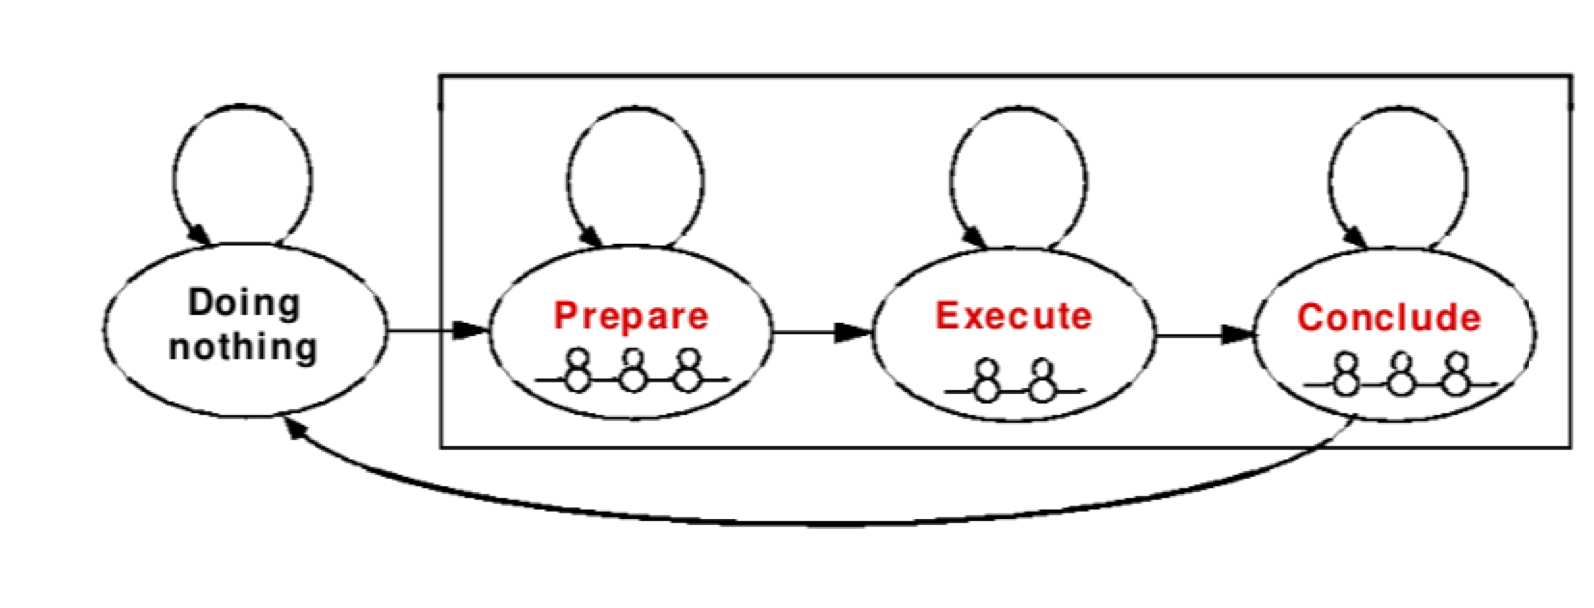
\includegraphics[width=120mm]{markov_model.png}
	\end{center}
	\caption{Basic schema of Markov model in human decision~\cite{patel}}
	\label{markovmodel}
\end{figure}\\
\textbf{Hidden Markov model} \label{subsec:hmm}\\
The statistical implementation of Markov chain in which the system being modeled is assumed to be a Markov process $X$ with unobservable states.
HMM assumes that there is another process $Y$ with dependent behavior on $X$.
This approach is used to learn about $X$ by observing $Y$.
The states of the process $X_n$ are hidden states and the result from equation:\\
\begin{equation} \label{eq:8}
P = (Y_n ∈ A|X_n = x_n),
\end{equation}\\
where $P$ is emission probability (sometimes called output probability) and $X_n$ is Markov process which is not directly observable.
Both $Y_n$ and $X_n$ be discrete-time processes, for every $n \geq 1, x_1,\ldots ,x_n$ and an arbitrary (measurable) set $A$.\\
This method is without any memory so past doesn't matter, only future is important and relevant for HMM.\\
\\
\textbf{A Markov model with social influences} \label{subsec:markov}\\
This model is based on Markov chains, an stochastic model describing a sequence of possible events in which the probability
of each event depends only on the state attained in the previous event.
A countably infinite sequence, in which the chain moves
state at discrete time steps, gives a discrete-time Markov chain (DTMC).
A continuous-time process is called a continuous-time Markov chain (CTMC).
It is named after the Russian mathematician Andrey Markov.
This method is actually better for our purpose than the time-continuous differential equations which are usually used for prediction.
In order to use this model approach, first of all we have to develop the possibility of a decoy effect.
Then we introduce sociology and obtain results for lock-in analogous.
These Markov models display both important similarities to and differences from the previous models, and may be simpler to work with.
The last but not the least pros of that models is very good graphical representation.\\
\\
\textbf{An Experiment Using Markov Dynamic Models} \label{subsec:markov_dynamic}\\
Shopping is natural-feeling and familiar type of human behavior that exhibits complex patterns that last from several seconds to several days.
These characteristics make shopping almost ideal experimental for modeling human behavior.
In the case of shopping, the macroscopic actions are events like needs, choosing brands, choosing seller.
The internal states are the individual steps that make up the action, and the observed variables will be changes during the shopping
process workflow in which can be decision of customer different.
The intuition is occasionally important, but this belongs to special market and marketing personal identification such a buying shoes by a single woman in production age.\\
\\
\textbf{Modeling and Prediction of Human Behavior may consist of the following steps:}\\
\begin{enumerate}
	\item needs decision to make,
	\item looking across the site to find some adequate product/service,
	\item make action decision,
	\item shopping workflow process in selected site,
	\item make final payment.
\end{enumerate}
\\
In this case psychology covers how and what influences people to make their choises of actual items on the shelves in
shop and the possible reason why they will buy something different from previously buyed.
Advertising might be comprised into these characteristics but could also possibly be considered as part of the sociological
influences (point 1 and 2), especially if the advertising takes the form of a well known figure endorsing a product.
More specifically, the following four properties have been identified by Unilever Research~\cite{patel} as being important and their influence were included in one or more models:

\begin{enumerate}
	\item Regret.
	This refers just two products compare with each other as regards different qualities, which can include price (or its inverse value).
	A customer might judge one item to be superior to another in all respects.
	\item Attribute change.
	The introduction of a new product onto the market can change the way of customers, or at least some of them, view established brands.
	This might be by drawing attention to some quality which was not previously much regarded, or it might make people give different
	weightings to the (established) qualities when making their decisions. The former can be considered to be a special case of the latter.
	\item Outlier avoidance.
	When a number of products are in many aspects quite similar, there can be a tendency for people to avoid ‘strange’ ones,
	like others which are substantially different from the majority in price or some other respect.
	Items near the average can be favoured.
	\item Decision process change.
	Decision process change.
	A straight choice between two items might be relatively easy.
	They can be compared according to price, size etc\. and a decision made. With three or more,
	comparisons might be made between two things at a time, one could be eliminated and then the winner contrasted with a third.
\end{enumerate}
\subsection{Viterbi algorithm} \label{subsec:viterbi}
The Viterbi algorithm~\cite{viterbi} is a dynamic programming algorithm for finding the most likely sequence of hidden states called
the Viterbi path that results in a sequence of observed events, especially in the context of Markov information
sources and hidden Markov models (HMM).\\
The algorithm has found universal application in decoding the convolutional codes used in both CDMA and GSM digital cellular,
dial-up modems, satellite, deep-space communications, and 802.11 wireless LANs.
Now it is also commonly used in speech recognition, speech synthesis, keyword spotting, computational linguistics, and bioinformatics.
For example, in speech-to-text (speech recogni- tion), the acoustic signal is treated as the observed sequence of events, and a string of text is considered
to be the "hidden cause" of the acoustic signal.
The Viterbi algorithm finds the most likely string of text given the acoustic signal~\cite{DBLP:journals/corr/abs-cs-0504020}. \\

\subsection{Predicted effects} \label{subsec:predicted}
\begin{enumerate}
	\item How a decoy product might influence the market.
	The appearance of a third product might remarkably change the market shares of two others, while getting minimal sales itself.
	This effect is one of the most complex biases in customer choice, and has been observed in product classes from chocolate bars to electronics to beer.
	The decoy effect illustrates the importance of customer psychology, to understand how customers recognize products, and how customers see quality side to buy the product.

	\item The dynamics of market share is how sales of products can change during the time.
	For example, even if two products are really equal in all relevant aspects, then after a long time of customer
	activity it might be that each product takes 50\% market share (preserving the symmetry), or one product takes
	nearly 100\% market share (breaking the symmetry), or that there is no steady state, with market dominance alternating between the two brands.
	The second of these three cases is called lock-in, corresponding to one brand obtaining a virtual monopoly, which is almost impossible to break.
	From that reason is not legally to create a monopole in some industries and for human purchase behavior is not good to calculate with monopole approach.

	\item How a new product will fare, given its quality profile compared with existing brands.
	This question is complementary to that of the decoy, asking what market share a new product will gain rather than how it will affect the market shares of existing products.

	\item A choice overload: when there are too many possible options for potential customers from which they can pick,
	many of them will search the sites without making a
	\item Minimise anticipated regret modelling property was taken to lead to simple comparisons along the lines of with regard to quality $k$,
	is product $i$ better than product $j$?
	If the answer to all relevant questions, $k = 1, . . . , nq$, if $nq$ is the number of qualities, is no, then a customer
	will not change from $j$ to $i$.
	The more times the answer is yes, the faster such a change is likely to happen.
\end{enumerate}
\\
\section{Customer preferences and decision process} \label{sec:customer_preferences}
Considering a customer whose preference is shared out amongst all the available brands in a market where there are no empty or zero brands,
so that the total of all brands preference shares is 1 (100\%).
The proportion of customer preference held by brand $X$ at time $t$ is denoted by $X(t)$.
For example, if the preference share of brand A is plotted against brand B in a market where only two brands exists,
the point must be somewhere along the straight line $B(t) = 1, A(t)$.
Of interest is the case when a third brand is added, possibly as a
The additional brand means that the preference distribution changes from being a straight line in the two-dimensional plane $(A, B)$,
to a plane in three-dimensional space $(A, B, C)$.\\
\\
\textbf{Customer decision process} \label{sec:cus_decision} described in~\cite{patel} show that the standard Logit model~\ref{subsec:logit} for customer choice assumes that
the probability, $p_i$, with which a customer buys a given product $i$ from a range of products $[1, n]$ depends on
the value which customer internally assigned to that product and his price.
This dependence is taken to be of exponential form.
Assuming that guaranteeing that all probabilities are positive)
\\
\begin{equation} \label{eq:9}
p_i = C\exp(V_i - sP_i),
\end{equation}
\\
where $s$ is a measure of the relative importance of price to the customer, and $C$ is a normalisation constant set to be results always positive. $V_i$ is subjective value
attached to product by a customer with dependency on price of the product $P_i$.~\cite{patel}:
\\
\begin{equation} \label{eq:10}
\sum_{i=1}^n p_i = 1.
\end{equation}
\\
The value $V_i$ is then taken to reflect the influence on the customer of the quality of the product,$Q_i$,
the increased likelihood of the customer buying the same brand as he bought previously (the loyalty effect),
and the peoples who have an influence on a customer (neighbours).
Each of these dependencies are taken to be linear, giving~\cite{patel}:
\\
\begin{equation} \label{eq:11}
V_i = aQ_i + lI_i + hN_i,
\end{equation}
\\
where $I_i$ is an indicator function which is unity if the customer a previously bought product i and zero otherwise,
$N_i$ is the number of neighbours who bought product $i$, and $a, l$ and $h$ are constants measuring the relative strength
of each effect.
In such a model the products are all treated independently.
Only coupling between the probabilities occurs through the normalisation constant $C$.
Product $I$ will depend not only on the value and price of that product, $V_i$ and $P_i$, but on the value and prices of all products.
The goal of this section is to formulate a model for this probability which is based on binary comparisons, that is,
on comparisons of two products at a time.\\
\subsection{Logit analysis in marketing} \label{subsec:logit}
Logit analysis is a statistical technique used by marketers to assess the scope of customer acceptance of a product, particularly a new product.
It attempts to determine the intensity or magnitude of customers' purchase intentions and translates that into a measure of actual buying behavior.
Logit analysis assumes that an unmet need in the marketplace has already been detected, and that the product has been designed to meet that need.
The purpose of logit analysis is to quantify the potential sales of that product.
It takes survey data on consumers purchase intentions and converts it into actual purchase probabilities.
Logit analysis defines the functional relationship between stated purchase intentions and preferences, and the actual probability of purchase.
A preference regression is performed on the survey data.
This is then modified with actual historical observations of purchase behavior.
The resultant functional relationship defines purchase probability.

\subsection{Brand or product changing} \label{subsec:brand}
We can mathematically express the process of decision to switch from one brand to another one.
Consider a linear flux $\alpha_{xy}$ of preferences moving to brand $X$ from brand $Y$.
All fluxes have to be strictly positive.
It's in improper to consider negative flux, so really excluded is only zero value.
Flux is the proportion of customer preference to switch to other brand or product from previous one.
\begin{figure}[h!]
	\begin{center}
		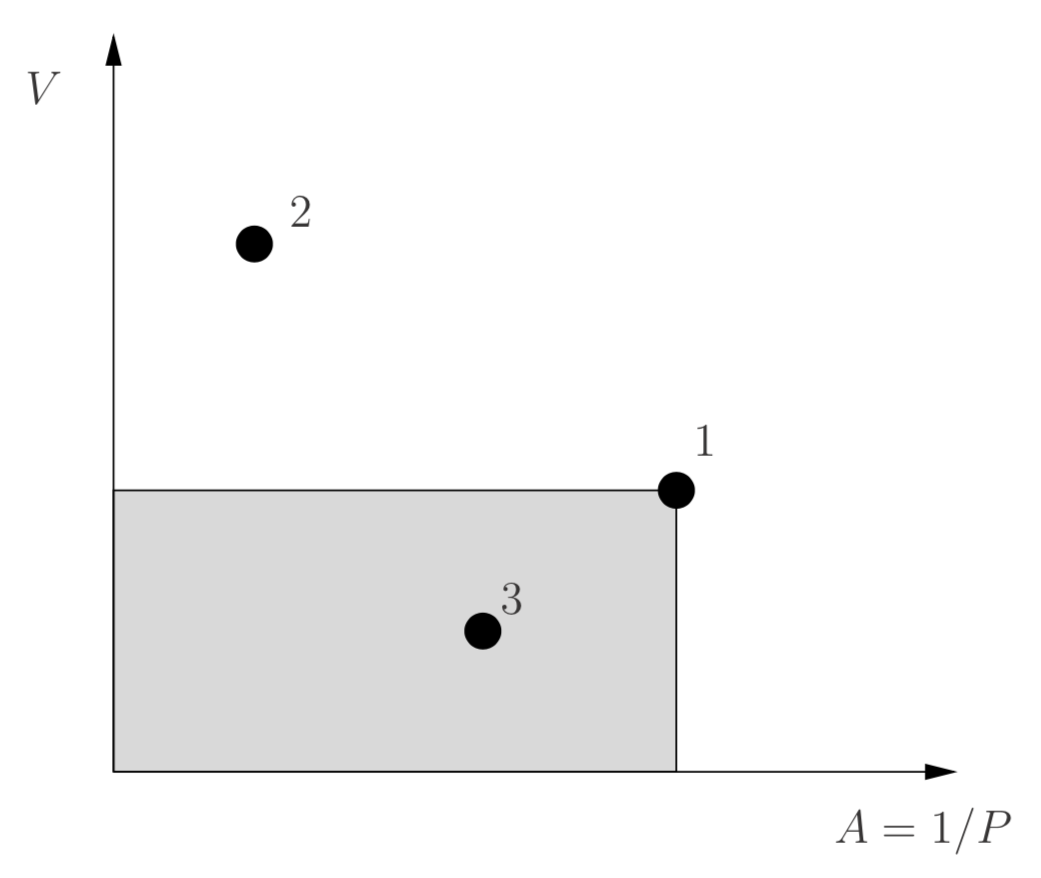
\includegraphics[width=80mm]{affordability.png}
	\end{center}
	\caption{Products in the affordability-value plane.
	The shaded region is the region of products dominated by product 1~\cite{pantland}.}
	\label{Affordability of products}
\end{figure}
\\
The basic idea from Models of Consumer Behaviour~\cite{patel} is to build a model based on a physical analogy,
between the customers buying behavior and particle-particle dynamics.
Let us assume customers to be particles moving in quality space.\\
\begin{figure}[h!]
	\begin{center}
		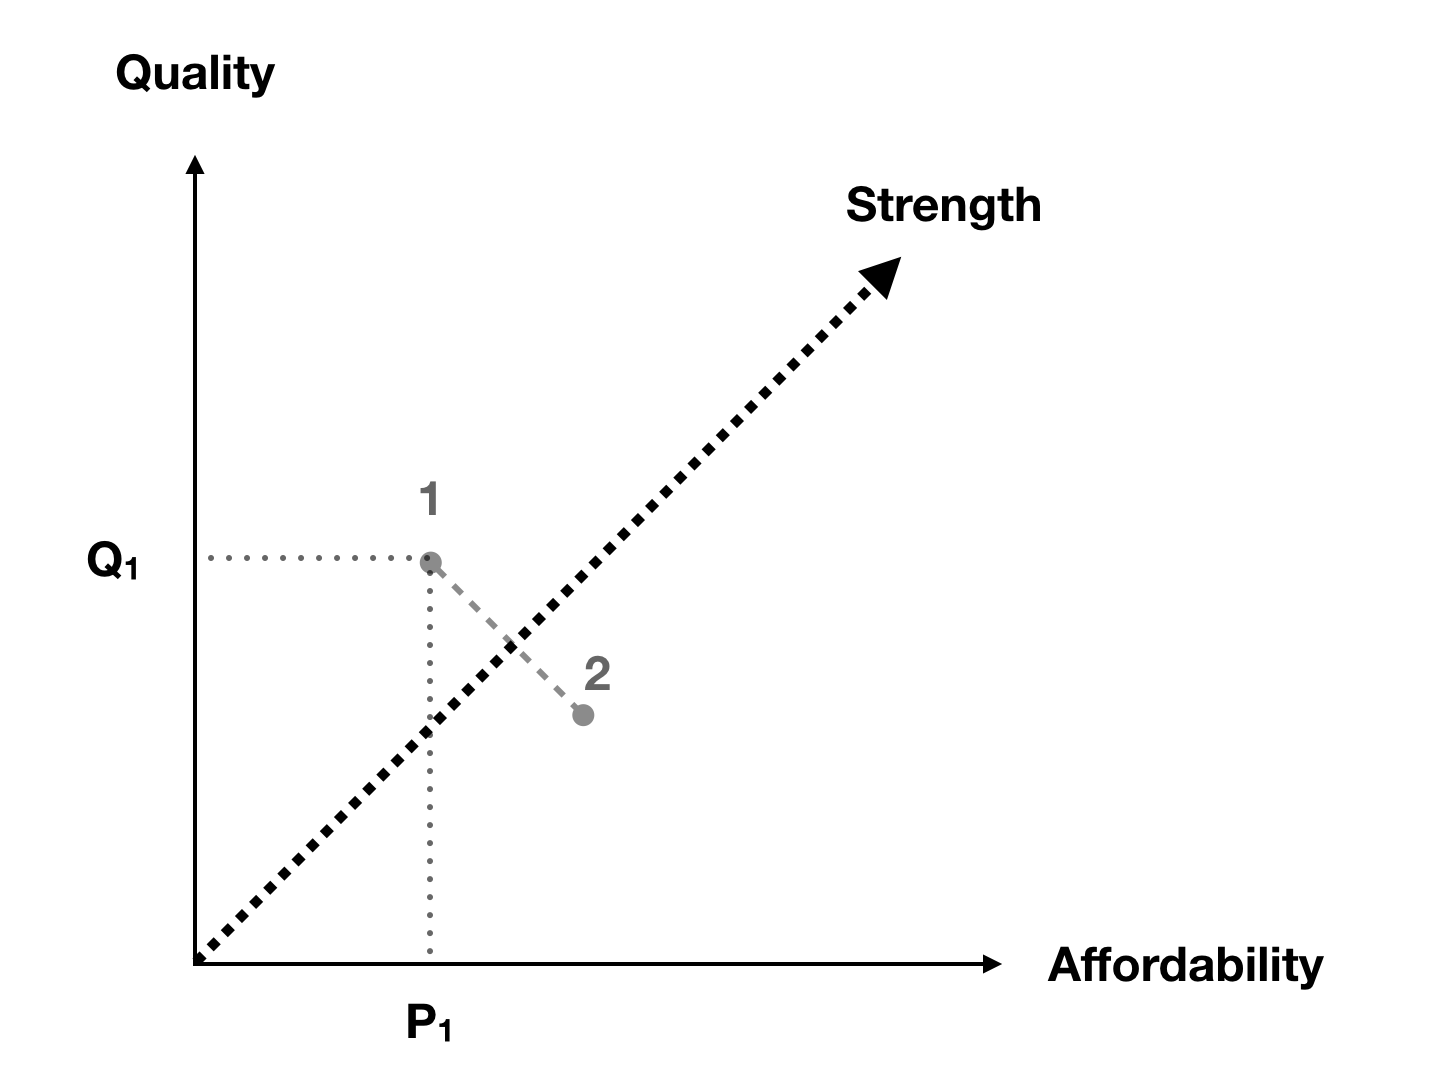
\includegraphics[width=80mm]{strength.png}
	\end{center}
	\caption{Product space with two products~\cite{patel}}
	\label{Strength of products}
\end{figure}
\\
The products are considered as sources of  potentials strength, the details of the potentials depending on the products’ characteristics.
The psychology of people will be regarded as the influence of the potential on the mass of the particles.
This will depend on the customer but also on the characteristics of each product, weighted by coefficients of choice.
The sociology of individuals can be considered as a form of particle-particle
Following what has gone before, the product space is defined by just two characteristics for each product $i$ with affordability $P_i$ and quality $Q_i$.
We can define the ‘strength’\footnote{The power if the product or service to be attractive for customer.} of a product as
the distance of the product from the origin in product space as~\cite{pantland}:
\\
\begin{equation} \label{eq:12}
U_i = \frac{(P_i + Q_i)}{2}.
\end{equation}
\\
All the products with $P_i + Q_i = constant$ will have the same strength.

% !TEX root = ../thesis.tex

\chapter{Syntactic part}
\label{sec:methodology}
\section{Goal of the work} \label{sec:goal}
Based on the analytical part~\ref{sec:analytical} we will be working on a mathematical models to predict customer behavior consist of vendor, psychology and loyalty sub-models combine in hidden markov model (HMM) to final prediction model.
States in the HMM will be read by viterbi algoritm~\ref{subsec:viterbi} which is able to predict most probability state in propagation by HMM.
We try to get a better results than actual standard statistical methods (Time Series analysis)~\ref{sec:statistics} to predict customer behavior in e-commerce.
In the final our model will be able to predict online store future income from previous income and number of visitors.
For successfully prediction we will use some open data for store strength and customer satisfaction and some predefined and computed variables from store.
\section{Modeling prediction of customer behavior} \label{sec:modeling}
The goal of model is to predict if customer will successfully finish order or leave store without make an order.
This model will be consists of three sub-models.
Vendor model,\ psychology model and loyalty model.
All sub-models will be combined to complex prediction mechanism, as you can see on image~\ref{Model schema with interaction}
To final prediction will be used Hidden Markov model in combination with Viterbi algorithm to detect hidden states to reflect set weights and get better results for each industry.
Weights for model are industry dependent and for my modeling we set them from Megaplay s.r.o data and with cooperation with the owner of Megaplay s.r.o who has more than 10 years of experience in that industry, so he is the right person to know that kind of business.
\\
\begin{figure}[h!]
    \begin{center}
        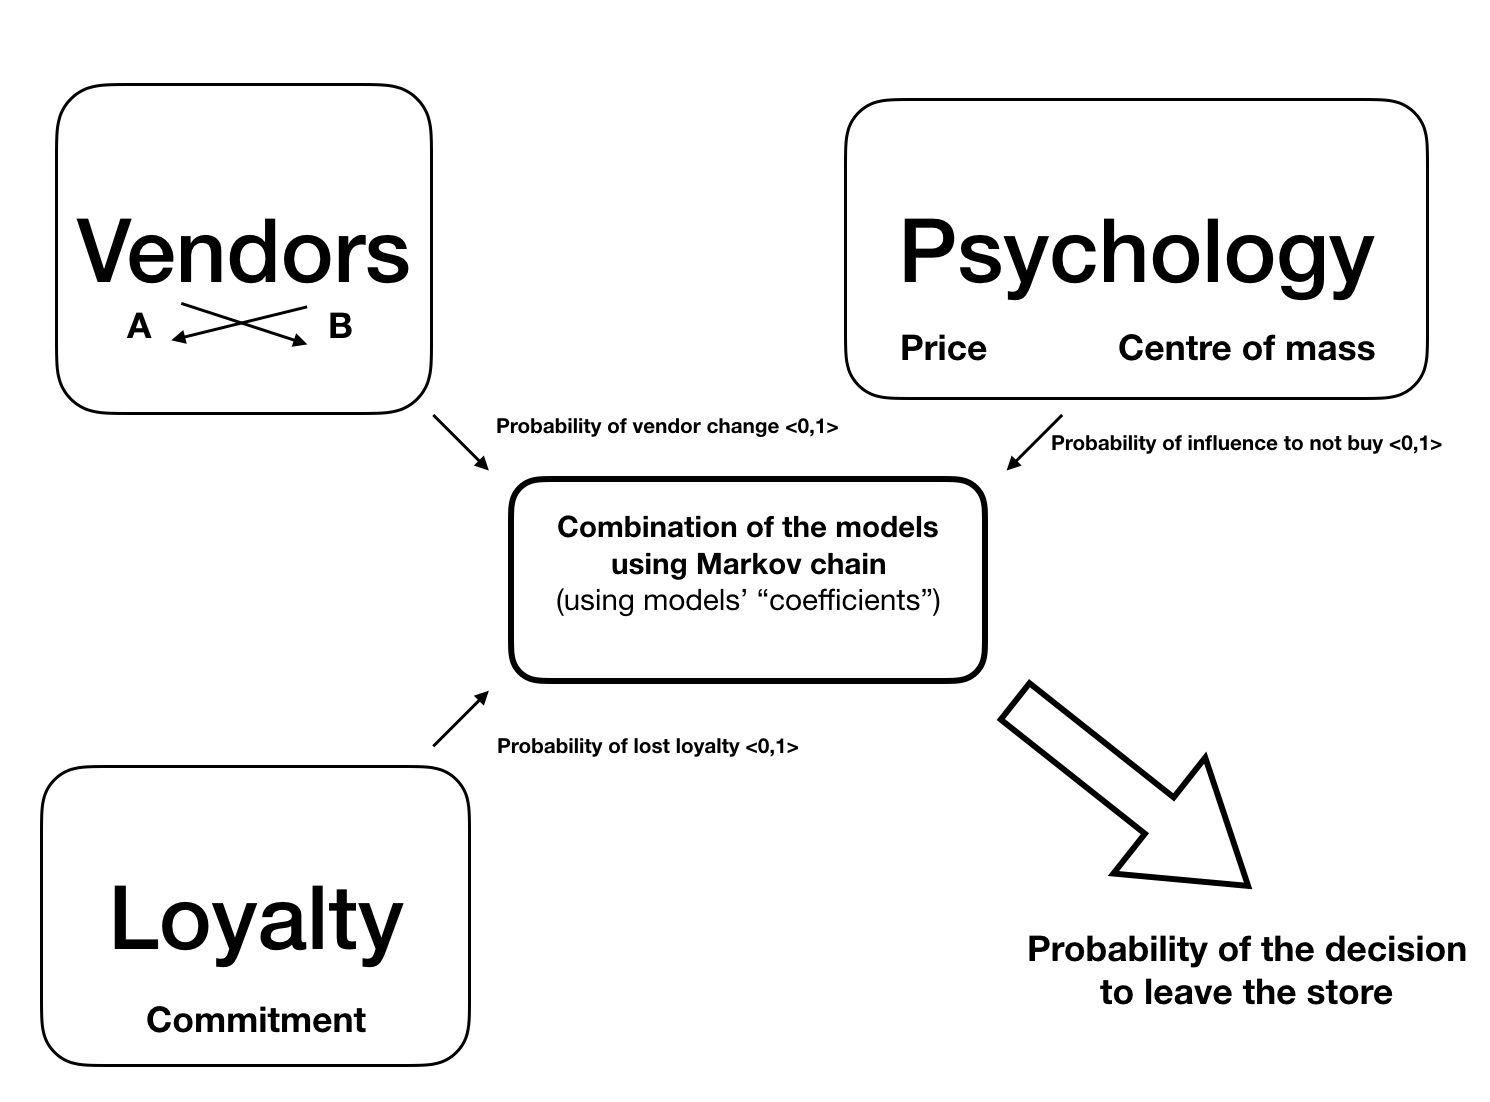
\includegraphics[width=140mm]{computation_schema.png}
    \end{center}
    \caption{Computation flow and interactions between models}
    \label{Model schema with interaction}
\end{figure}
\\
\subsection{Preprocessing of input data} \label{subsec:preprocessing}
Data should have to be anonymize \footnote{Data anonymization is a type of information sanitization whose intent is privacy protection.
It is the process of either encrypting or removing personally identifiable information from data sets, so that
the people whom the data describe remain anonymous.} and pseudonymized \footnote{Pseudonymization is a data management
and de-identification procedure by which personally identifiable information fields within a data record are replaced
by one or more artificial identifiers, or pseudonyms.} to keep legal notice of~\cite{gdpr}.
Then we should utilize data to utilized inputs.
This prepared data I will add to the Matlab live script file to be used for prediction.\\
\\
\textbf{Average day visitors for a predicted month}\\
This value was calculated from anonymize user data from Google Analytics tool used their prediction mechanism to get number of future users based on previous a number of visitors.\\
\\
\textbf{Perceived value for psychology model} \label{perceived}\\
This variable is needed for loyalty model~\ref{subsec:model_loyalty} and comes from an open e-commerce compare data provided by Heureka.cz/Heureka.sk internal tool.\\
\\
\textbf{Number of orders 2018 - 2019}\\
Number of orders get from shopycrm.com tool used in Megaplay s.r.o to manage their business processes and store all needed data.\\
\\
\textbf{Unique products sell}\\
This variable is used in Psychology model~\ref{subsec:model_psychology} for Price aspect calculation~\ref{eq:26}.\\
\\
\textbf{Customer satisfaction} \label{customerSat}\\
This value is provided by Heureka open data, and it's a calculated value from the all customer reviews of the store.\\
\\
\textbf{Margin}\\
The retail margin percentage measures the retail margin as a percentage of the retail price.
This measurement gives you a context for the retail margin.
For example, if you have a 5~€ retail margin on two different products, but one costs 150~€ and next one costs 10~€, the second product would have a much higher retail margin percentage.\\
\\
\textbf{Number of product order each day $Q_i$}\\
This is a calculated value from shopycrm.com about number of product order for each one.
It's used in Psychology model~\ref{subsec:model_psychology}. \\
\\
\textbf{Quality index $Q_1$}\\
This is vendor quality index provided by Heureka open data.
This is a power/strength of the store.
Higher number mean that for a customer is more difficult to leave the store and go to another online store.\\
\\
\textbf{Vendor coefficients $\beta, \gamma, \delta$} \label{vendorCoeff}\\
This three coefficients are used as weight for vendor model~\ref{subsec:model_vendors} and was set with cooperation with Megaplay s.r.o owner for their industry.
It's represent the relation between vendor prices and vendor quality.\\
\\
\begin{table}[h!]
    \begin{center}
        \begin{tabular}{ | l | c |}
            \hline
            {\textbf{Variable name}} & \textbf{Value}\\
            \hline
            average day visitors for a predicted month $U_a$& 2357 \\
            perceived value for psychology model & 0.87 \\
            number of orders 2018 - 2019 $O_c$ & 26 530 \\
            Unique products sell $U_p$ & 11048\\
            Customer satisfaction & 90\%\\
            Margin & 0.27\\
            $Q_i$ & 4.12\\
            $Q_1$ & 0.94\\
            Vendor coefficients: & \\
            $\beta$ & 0.7\\
            $\gamma$ & 0.7\\
            $\delta$ & 0.85\\
            \hline
        \end{tabular}
    \end{center}
    \caption{Coefficient data from Megaplay s.r.o}
    \label{megaplay_data}
\end{table}
\\
\begin{table}[h!]
    \begin{center}
        \begin{tabular}{ | l | c |}
            \hline
            {\textbf{Variable name}} & \textbf{Value equation}\\
            \hline
            number of visitors 1/2020 & $31 * U_a$\\
            average earn per order & $\sum EARN / O_c$\\
            \overline{Q} & $1/U_p * (U_p/ O_c)$\\
            \overline{P} & $1/U_p * margin$\\
            trust & $1/O_c * O_c/U_a$\\
            \hline
        \end{tabular}
    \end{center}
    \caption{Calculated data from Megaplay s.r.o}
    \label{megaplay_data_equation}
\end{table}
\\
\subsection{Vendors} \label{subsec:model_vendors}
For simplification, we will take to account only a two vendors market share, without 100\% domination, because of on a real
market is 100\% monopole unlikely see and then we will be reflected only main competitor.
From that condition it is evident that for market dominate vendor it will return false positive results.
Our model is based on equations from Brands section~\ref{eq:10} and from those equations we will get probability of vendor change from
vendor $A$ to vendor $B$ and if the vendor $B$ will have more strength than vendor $A$ it will break the computation and customer
will leave our store without successfully completing buy process.
Results of this computation wil be probability for each iteration of buy process simulation in an interval $<0,1>$.
Data for this model will comes from open data provided by google.com, heureka.cz/heureka.sk and national governments.
That data will be combined with calculated price indexes downloaded from shopycrm.com tool.
\\
\begin{equation} \label{eq:24}
\alpha_{xy} = \beta H(P_x-P_y) + \gamma H(Qx-Qy) + \delta H(Px-Py)H(Q_x - Q_y)
\end{equation}
\\
where $\beta, \gamma, \delta$ are non-negative~\ref{vendorCoeff}.
\\
\begin{itemize}
    \item $P$ is prices of vendors products
    \item $Q$ is a quality index of vendor
    \item $H$ is a Heaviside function which will be calculated by~\ref{eq:22}.
\end{itemize}
\\
\begin{eqnarray} \label{eq:25}
H(s) = 1, s > 0 \\
H (s) = 0, s \leq 0
\end{eqnarray}
\\
\subsection{Psychology} \label{subsec:model_psychology}
Psychology aspect is trying to simulate customer behavior in thee situation like a prices aspect, society influenced, mood aspect, actual needs
and so on.
In this model we will simplify only for price effect~\ref{subsubsec:model_psychology_price} and center of mass effect~\ref{subsubsec:model_psychology_mass}
\subsubsection{Price aspect} \label{subsubsec:model_psychology_price}
\begin{equation} \label{eq:26}
\overset{-}{Q} = \frac{1}{n_p} \sum_{i=1}^{n_p} Q_i
\end{equation}
\\
\begin{itemize}
    \item $Q_i$ number of orders for product $i$ per day divide amount of orders per same day, prom interval $<0,1>$
    \item $n_p$ number of products in store
\end{itemize}
\\
\begin{equation} \label{eq:27}
\alpha_{ij} = \frac{C+max(Q_j, \overset{-}{Q})}{C+max(Q_i, \overset{-}{Q})}
\end{equation}
\\
Coefficient C is used to be $\alpha_{ij}$ always positive.
\subsubsection{Center of mass aspect} \label{subsubsec:model_psychology_mass}
Center of mass aspect is applied as a part of sociology to our psyhology model.
Marketers use it to manipulate with customers in global way.
Like a black friday, Cyber monday etc., in that days stores manipulate with our psychology by discount prices.
\\
\begin{equation} \label{eq:28}
\overset{-}{P} = \frac{1}{n_p} \sum_{i=1}^{n_p} P_i
\end{equation}
\begin{itemize}
    \item $P_i$ is defined as product price minus retail recommend price divide average price
    \item $n_p$ number of products in store
\end{itemize}
\\
\begin{equation} \label{eq:29}
\alpha_{ij} = \frac{C+max(P_j, \overset{-}{P})}{C+max(P_i, \overset{-}{P})}
\end{equation}
\\
This model returns probability for customer decision to make action from interval $<0,1>$.
\\
\subsection{Loyalty} \label{subsec:model_loyalty}
This models is based on Luarn & Lin research~\cite{luarn} and we change theirs model for our needs.\\
\begin{equation} \label{eq:30}
L = \frac{R+Z}{Z}
\end{equation}
\\
\begin{enumerate}
    \item L ..... probability of whole loyalty model
    \item R ..... probability of separate loyalty model
    \item Z ..... probability of commitment model
\end{enumerate}
\\
As we see on~\ref{Loyalty scheme} Loyalty model is consist of all three sub-models (Trust, Customer Satisfaction, Perceived value)
but commitment model consist of only Trust and Customer Satisfaction.
a,b,c,d,e .... weight coefficient to combine Trust, Customer satisfaction and Perceived value.\\
\newpage
Trust
\begin{equation} \label{eq:31}
T = \frac{1}{n} \sum_{i=1}^{n} O_i
\end{equation}
\\
$O_i$ number of orders divide number of visitors per day $i$
\\
\\
\textbf{Customer satisfaction}~\ref{customerSat} are datasets get from open data per each day, individual satisfaction.
For simplified the situation we will use average satisfaction per whole store.
\textbf{Perceived value}~\ref{perceived} is subjective value, which depend on a strength of the store.
\subsubsection{Commitment and Loyalty} \label{subsubsec:model_loyalty_commitment}
\textbf{Commitment} is making the actual choice every day or other period basis to keep up with something e.g. a relationship, personal goal, a task, etc.
We would have to hold ourself accountable to keep a commitment to something or someone.
Similarly, being loyal involves holding ourself accountable as well.
Against of \textbf{Loyalty} which is usually seen as a character trait rather than a conscious decision.
This model return probability for customer decision to not leave the store from interval $<0,1>$.\\
\\
\begin{figure}[h!]
    \begin{center}
        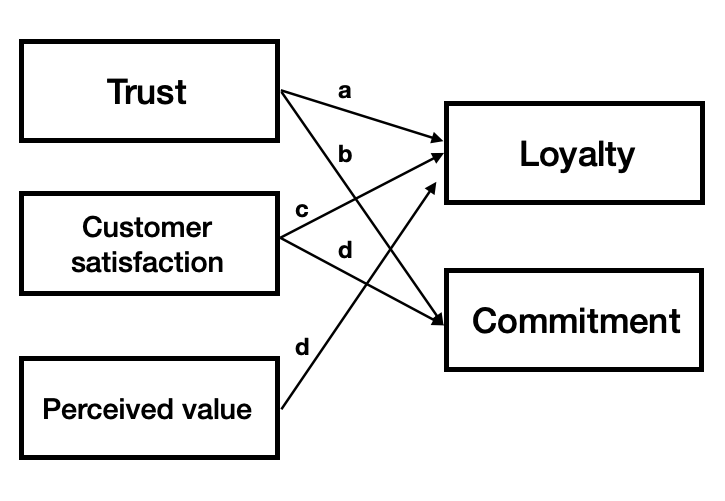
\includegraphics[width=140mm]{loyalty.png}
    \end{center}
    \caption{Computation flow for loyalty and commitment}
    \label{Loyalty scheme}
\end{figure}
\subsection{Combining models to decision process} \label{subsec:combining_models}
All separates models return probabilities vectors which we update to square matrix which is use as input to Hidden Markov model (HMM) \footnote{Hidden Markov Model (HMM) is a statistical Markov model
in which the system being modeled is assumed to be a Markov process with unobservable (i.e. hidden) states.
The hidden Markov model can be represented as the simplest dynamic Bayesian network.
The mathematics behind the HMM were developed by L. E. Baum and coworkers.
HMM is closely related to earlier work on the optimal nonlinear filtering problem by Ruslan L. Stratonovich,
who was the first to describe the forward-backward procedure.}
These probabilities will be combined with specific weights coefficients to always prevent positives results.
\section{Decision process from sub-models} \label{sec:decision}
\subsection{Hidden markov model} \label{subsec:hhm}
In a Hidden Markov Model (HMM), we have an invisible Markov chain (which we cannot observe), and each state
generates in random one out of $k$ observations, which are visible to us. Let’s look at an example.
Suppose we have the Markov Chain from above, with three states (snow, rain and sunshine),
$P$ - the transition probability matrix and $q$ — the initial probabilities.
This is the invisible Markov Chain — suppose we are home and cannot see the weather.
We can, however, feel the temperature inside our room, and suppose there are two possible observations: hot and cold.\\
For our need we will create 3 states model.
States will be:\\
\begin{itemize}
    \item order
    \item not finished order
    \item no order decision
\end{itemize}
With Megaplay s.r.o owner and heureka e-comerce tool calculation data we were set probability wages vector for HMM function like:\\
$$ p_w = \left(\frac{1}{3} & \frac{1}{2} & \frac{1}{9}\right) $$
\\
Vector have to be updated to square matrix which is used in HMM function.\\
\begin{equation*}
    P_w =
    \begin{pmatrix}
        \frac{1}{3} & \frac{1}{2} & \frac{1}{9} \\
        \frac{1}{3} & \frac{1}{2} & \frac{1}{9} \\
        \frac{1}{3} & \frac{1}{2} & \frac{1}{9}
    \end{pmatrix}
\end{equation*}\\
\\
\subsection{Used software, libraries and predefined functions} \label{subsec:libraries}
\textbf{Matlab 2020a}\\
MATLAB (matrix laboratory) is a fourth-generation high-level programming language and interactive environment for numerical
computation, visualization and programming developed by MathWorks.\\
\\
\textbf{Matlab LiveScript}~\cite{livescript}\\
MATLAB live scripts and live functions are interactive documents that combine MATLAB code with formatted text, equations,
and images in a single environment called the Live Editor.
In addition, live scripts store and display output alongside the code that creates it.\\
Use live scripts and functions to:\\
\begin{itemize}
    \item Visually explore and analyze problems
    \item Share richly formatted, executable narratives
    \item Create interactive lectures for teaching
\end{itemize}\\
\\
\textbf{hhmgenerate}~\cite{hhmgenerate}\\
The function $hmmgenerate$ begins with the model in state 1 at step 0, prior to the first emission.
The model then makes a transition to state $i_1$, with probability $T_{1i_1}$, and generates an emission $a_k_1$ with probability $E_{i_1k_11}$.
$hmmgenerate$ returns $i_1$ as the first entry of states, and $a_k_1$ as the first entry of seq.
$[seq,states] = hmmgenerate(len,TRANS,EMIS)$ takes a known Markov model, specified by transition probability matrix $TRANS$ and emission probability matrix $EMIS$,
and uses it to generate:\\
\begin{itemize}
    \item A random sequence seq of emission symbols
    \item A random sequence states of states
\end{itemize}
The length of both $seq$ and $states$ is $len$.
$TRANS(i,j)$ is the probability of transition from state $i$ to state $j$.
$EMIS(k,l)$ is the probability that symbol $l$ is emitted from state $k$.\\
\\
\textbf{hhmviterbi}~\cite{hhmviterbi}\\
The function $hmmviterbi$ begins with the model in state 1 at step 0, prior to the first emission.
hmmviterbi computes the most likely path based on the fact that the model begins in state 1.
$STATES = hmmviterbi(seq,TRANS,EMIS)$ given a $sequence, seq$, calculates the most likely path through the hidden Markov model
specified by transition probability matrix, $TRANS$, and emission probability matrix $EMIS$. $TRANS(i,j)$ is the probability of transition from state $i$ to state $j$.
$EMIS(i,k)$ is the probability that symbol $k$ is emitted from state $i$.\\
\\
\textbf{shopycrm.com}\\
Online CRM application focused on e-commerce stores which provides all store workflows and get precalculated data which we will use for our models to simplify the prediction calculation.
\newpage
\section{Time series for setting reference values} \label{sec:timeseries}
Based on statistical solution chapter~\ref{sec:statistics} we create four statistical approaches to predict 1/2020 income for store based on previous data from years 2018 and 2019.
This previous income can be found in appendix A Reference data~\ref{reference_data}.
To have a better idea about a point of view look on graph~\ref{income} with income data.\\
\begin{figure}[h!]
    \begin{center}
        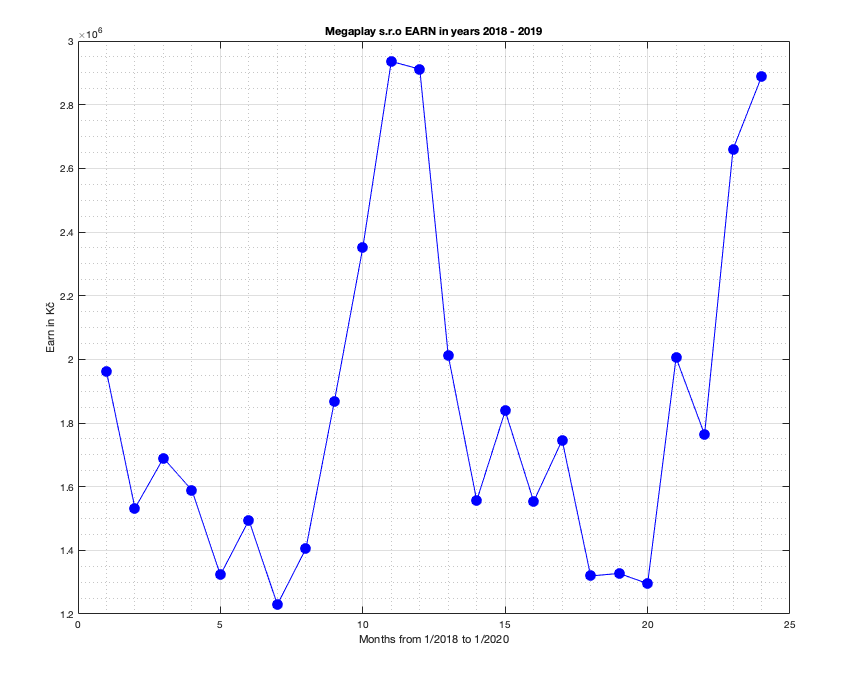
\includegraphics[width=150mm]{income.png}
    \end{center}
    \caption{Megaplay s.r.o income from stores in 2018 - 2019}
    \label{income}
\end{figure}
\subsubsection{Moving average}
Like a first basic time series analysis we tried moving averages.
This method looks like not useful for our needs, because of not able to reflecting trend in
specific e-commerce trends as Christmas time and new years discounts.
For our prediction reference data we will create prediction with moving average $n=3$ and $n=5$.
Here you can see part of code in Matlab to create the prediction, than you can see results in graph~\ref{moving_average_3}
for $n=3$ and on the next graph~\ref{} for $n=5$\\
\\
\textbf{Calculation for n=3}\\
\begin{lstlisting}[language=mcode]
% generate matrix for moving average n=3
% EARN is matrix with income data per months
for i = 2:length(EARN)
    if i < 24
        average3(1,i-1) = (EARN(1, i-1)+EARN(1, i)+EARN(1,i+1))/3;
    end
end

% with wages 1/4 1/2 1/4
for i = 2:length(EARN)
    if i < 24
        average3wages(1,i-1) = (1/4*EARN(1, i-1))+ ...
        (1/2*EARN(1, i))+(1/4*EARN(1,i+1));
    end
end

% moving average n=3 first level prediction
firstLevelPrediction = 1/3*(-2*EARN(1,22)+1*EARN(1,23)+4*EARN(1,24))
\end{lstlisting}\\
\\
Result from this prediction for 1/2020 is 3 561 213 Kč and it's aberration is 41.88\%.\\
\\
\textbf{Calculation for n=5}\\
\begin{lstlisting}[language=mcode]
% generate matrix for moving average n=5
% EARN is matrix with income data per months
for i = 3:length(EARN)
    if i < 23
        average5(1,i-2) = (EARN(1, i-2)+EARN(1, i-1)+EARN(1, i)+ ...
        EARN(1,i+1)+EARN(1, i+2))/5;
    end
end

% with wages 1/35(-3,12,17,12,-3)

for i = 3:length(EARN)
    if i < 23
        average5wages(1,i-2) = 1/35*(-3*EARN(1, i-2)+ ...
        12*EARN(1, i-1)+17*EARN(1, i)+12*EARN(1, i+1)-3*EARN(1, i+2));
    end
end

% first level prediction for n=5
firstLevelPrediction5 = 1/10*(-4*EARN(1,20)-1*EARN(1,21)+...
                        2*EARN(1,22)+5*EARN(1,23)+8*EARN(1,24))
% second level prediction for n=5
secondLevelPrediction5 = 1/5*(3*EARN(1,20)-3*EARN(1,21)-...
                        4*EARN(1,22)+0*EARN(1,23)+9*EARN(1,24))
\end{lstlisting}\\
\\
Result from this prediction for 1/2020 are 3 274 399 Kč and it's aberration is 33.91\% for first level prediction and 3 361 156 Kč with aberration 30.45\%.\\
\begin{figure}[h!]
    \begin{center}
        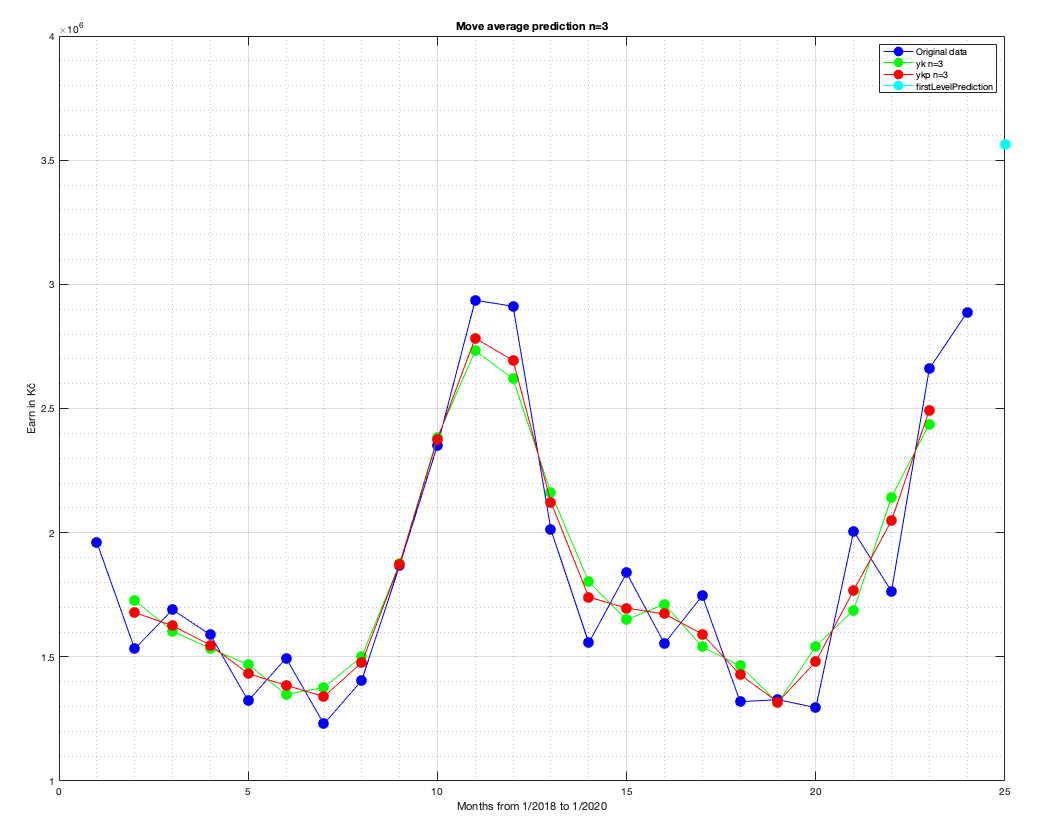
\includegraphics[width=150mm]{moving_average_3.png}
    \end{center}
    \caption{Moving average results for n=3}
    \label{moving_average_3}
\end{figure}
\begin{figure}[h!]
    \begin{center}
        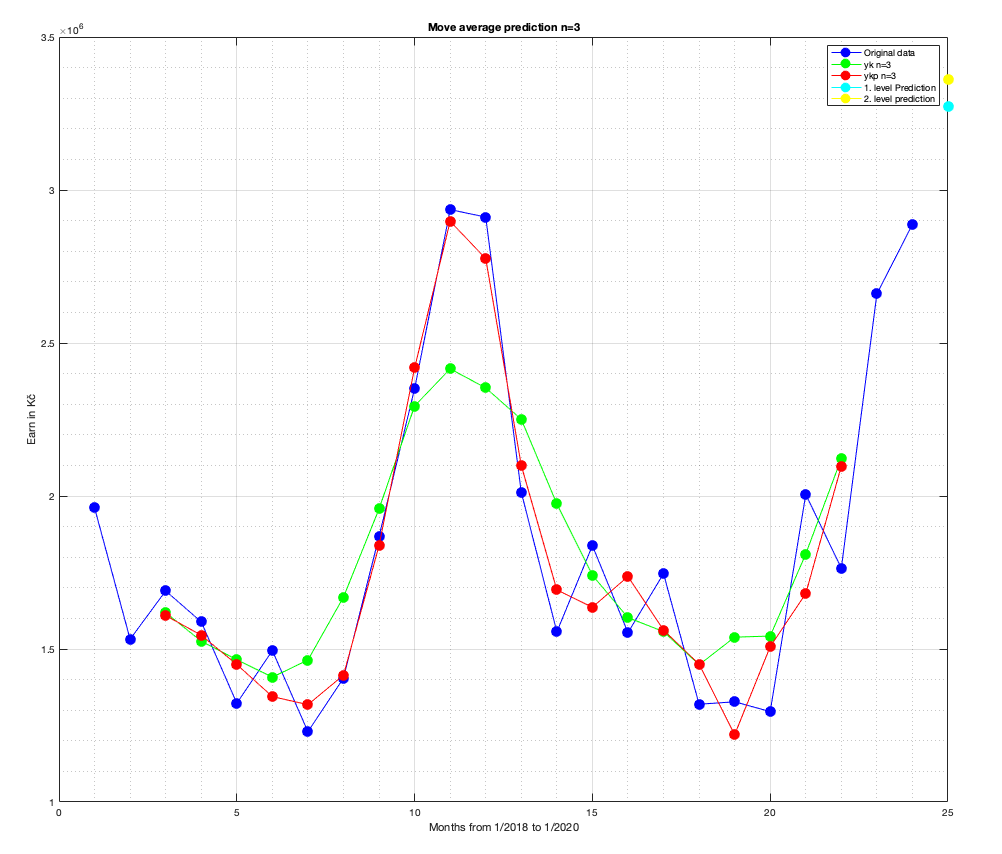
\includegraphics[width=150mm]{moving_average_5.png}
    \end{center}
    \caption{Moving average results for n=5}
    \label{moving_average_5}
\end{figure}
\subsubsection{Models}
After moving average we use two models for linear regression to predict other reference data by better statistical solutions.
We will use these two models:
\begin{itemize}
    \item $Tr_{t1}=a_0+a_1t$
    \item $Tr_{t2}=a_0+a_1t+a_2t^2$
\end{itemize}\\
\\
\textbf{Regression analysis for $Tr_{t1}=a_0+a_1t$}\\
\begin{lstlisting}[language=mcode]
X = [ones(1,24); ...
1:1:24];
XTX = X*X';
invXTX = inv(XTX);
XTY = X*EARN';
parameters = invXTX*XTY;
a0 = parameters(1, 1);
a1 = parameters(2, 1);
Trt1 = a0+a1.*t;

%prediction for 1/2021
PredictionTrt1 = a0+a1*25
\end{lstlisting}\\
\\
\textbf{Regression analysis for $Tr_{t2}=a_0+a_1t+a_2t^2$}\\
\begin{lstlisting}[language=mcode]
X2 = [ones(1,24); ...
    1:1:24; ...
    1^2 2^2 3^2 4^2 5^2 6^2 7^2 ...
    8^2 9^2 10^2 11^2 12^2 13^2 14^2 15^2 16^2 ...
    17^2 18^2 19^2 20^2 21^2 22^2 23^2 24^2];
XTX2 = X2*X2';
invXTX2 = inv(XTX2);
XTY2 = X2*EARN';
parameters = invXTX2*XTY2;
a0 = parameters(1, 1);
a1 = parameters(2, 1);
a2 = parameters(3, 1);
Trt2 = a0+a1.*t+a2.*t.^2;

%prediction for 1/2020
PredictionTrt2 = a0+a1*25+a2*25^2
\end{lstlisting}\\
\\
We got better results from model $Tr_{t2}=a_0+a_1t+a_2t^2$ as you can see on graph~\ref{ts_models}.
The goal of this thesis is not about to find the best statistical solutions in time series, so for our purpose this model is enough as a reference.
Time series analysis for better model have the results with aberration of 14,56\% from the real 2020 income.
All models result you can see in evaluation part~\ref{evaluation}.\\
\begin{figure}[h!]
    \begin{center}
        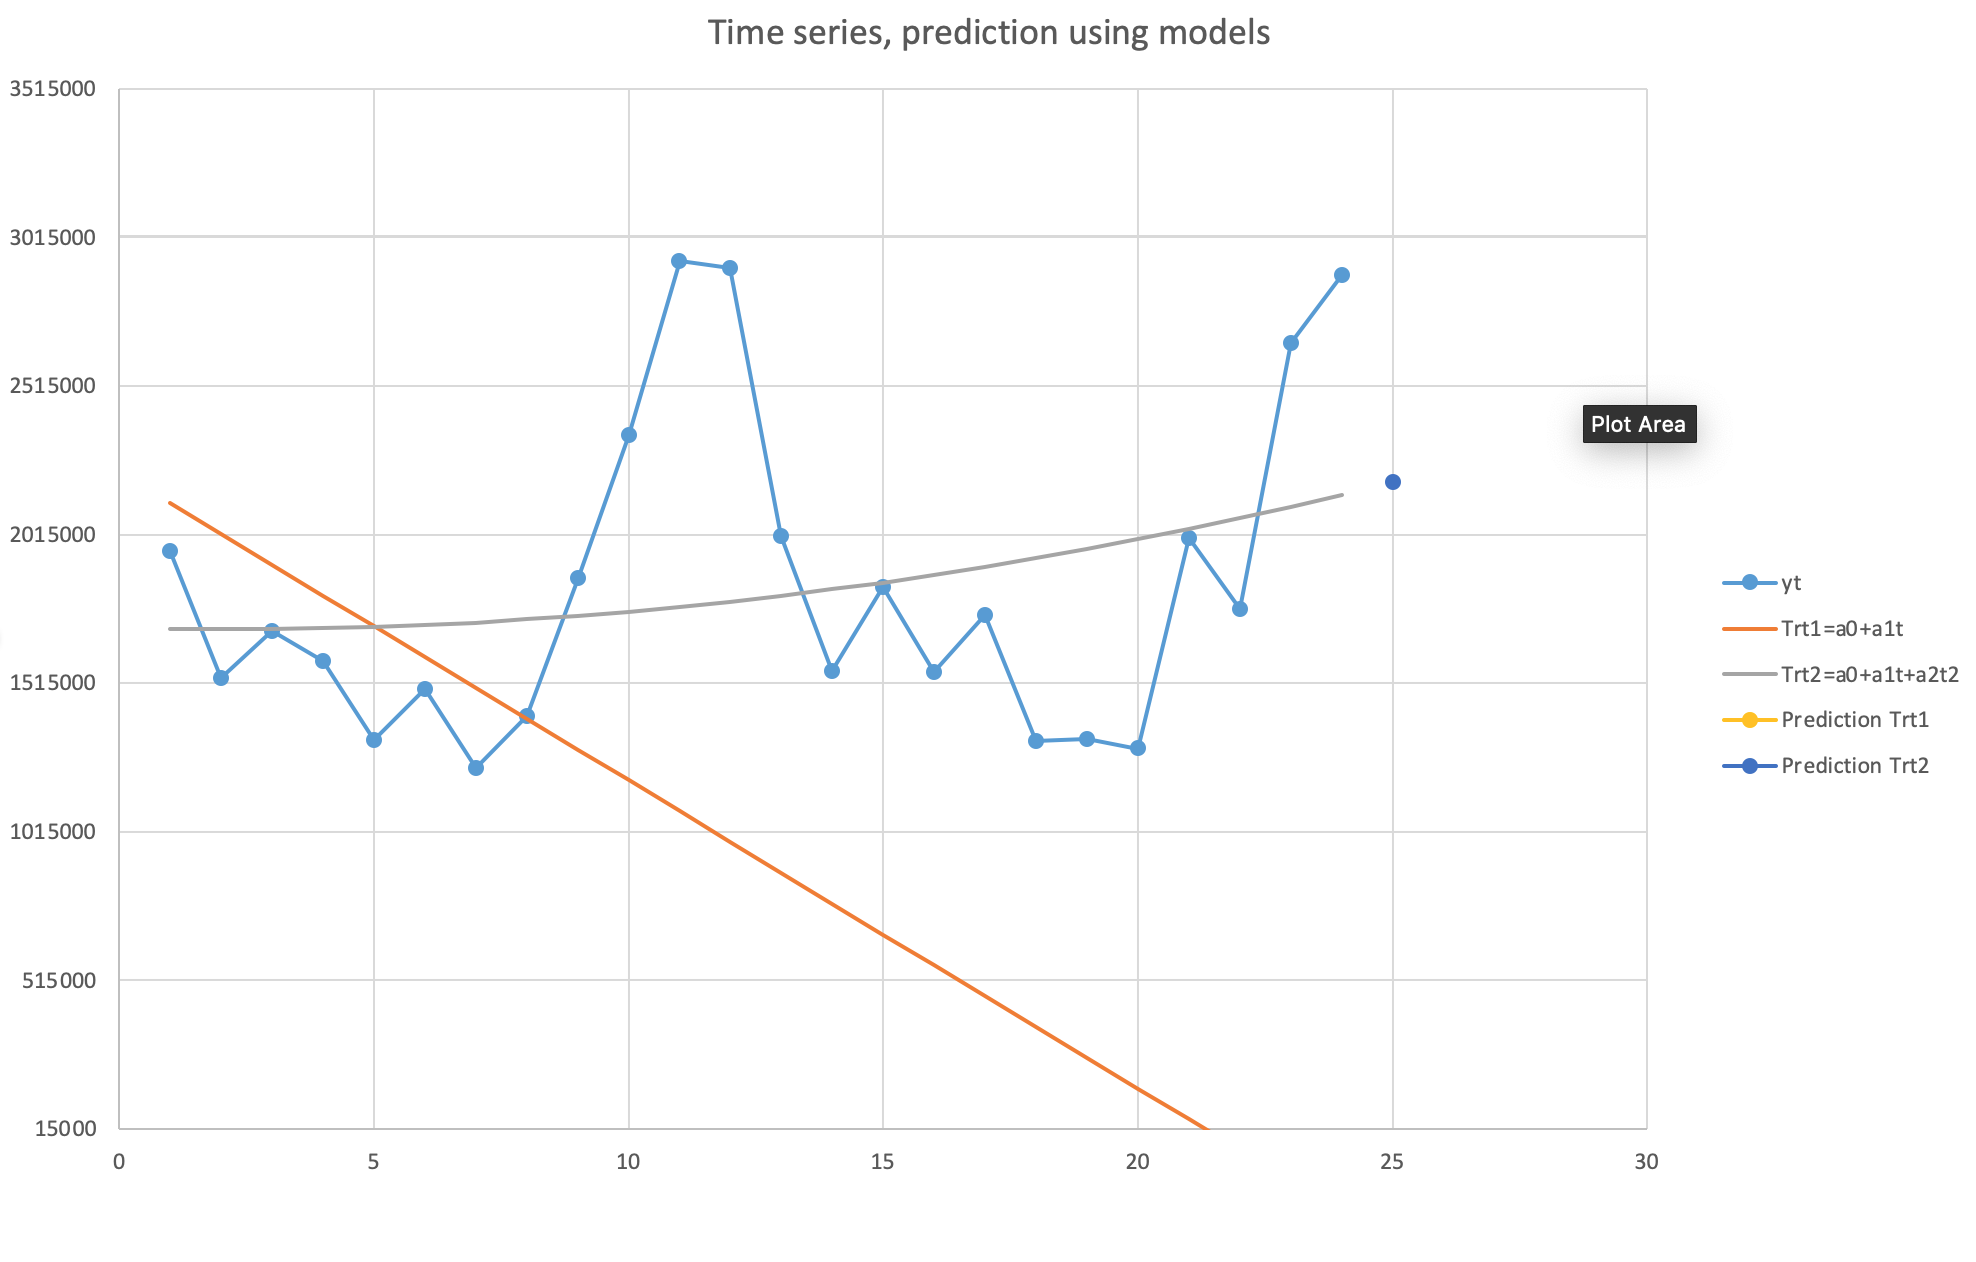
\includegraphics[width=140mm]{model_ts.png}
    \end{center}
    \caption{Time series model results}
    \label{ts_models}
\end{figure}
\newpage
\section{Prediction application} \label{sec:app}
Our prediction script is finally written in Matlab Live script with predefined constants based on Megaplay s.r.o data,
but for modeling and dynamic prediction are used Live scripts Controls so in the script we are able to easily set all constant to model for simulate different situations. We can see model situation in~\ref{appendixc} and taht results is described in the final summary~\ref{summary}.\\
\subsection{Using random values} \label{subsec:rand}
In our model we use random generated variables to simulate situations from real store where the user can compare with other store in the different situation.
This other stores and situation should be better or worst to actual store.
\subsection{Main Matlab code} \label{subsec:matlab}
\begin{lstlisting}[language=mcode]
% generate 10 times for get average values to prevent
% false positive and negative results
for c=1:experimentationCycles
    % go with each visitor thrue the prediction model and get
    for i=1:numberOfVisitors1_2020
        % actual tested value for each cycle
        Pj = generatePriceOfProduct();
        % product price minus product retail price
        Pi = Pj*margin;
        % actual product order value for each cycle
        Qj = 1;
        % statistic value get from open data
        if rand(1) > 0.98
            % Quality index for vendor 2
            Q2 = Q1 - rand(1);
            % vendor 2 product price
            P2 = Pj  - rand(1);
            satisfaction = customerSatisfaction - randi(10);
        else
            % Quality index for vendor 2
            Q2 = Q1 + rand(1);
            % vendor 2 product price
            P2 = Pj + rand(1);
            satisfaction = customerSatisfaction+randi(10);
        end
        % get value of vendor submodel
        vendorProbability = vendor(beta, gamma, delta,...
                            Pj, P2, Q1, Q2);
        % get value of psychology submodel
        psychologyProbability = psychology(averageP,...
                averageQ,Pj, Pi, Qj, Qi);
        % get value of loyalty submodel
        loyaltyProbability = loyalty(satisfaction,...
                trust, perceived);
        % customer goes to other online store
        % go to next cycle
        if vendorProbability == 0
            continue
        end

        % prepare square matrix for hidden markov model
        trans = [vendorProbability vendorProbability ...
        vendorProbability; psychologyProbability ...
        psychologyProbability psychologyProbability; ...
        loyaltyProbability loyaltyProbability ...
        loyaltyProbability];

        % generate hidden markov model data
        [seq,states] = ...
            hmmgenerate(3,trans,probabilityWages,...
                'Statenames',{'order';'not finished order';...
                'no order decision'});

        % use viterbi algoritm to get states during hmm
        estimatesStates = ...
            hmmviterbi(seq,trans,probabilityWages,...
                'Statenames',{'order';'not finished order';...
                'no order decision'});

        % check states that customer not finished order
        exactMatchMask = strcmp(estimatesStates,...
                'no order decision');

        if  sum(exactMatchMask) < 1
            orders = orders + 1;
            % increate psychology effect of success store
            % when order is finished
            Qj = Qj + 1;
        end
    end
end
\end{lstlisting}\\
\subsection{Sub-models function in Matlab} \label{subsec:matlab-sub-models}
\begin{lstlisting}[language=mcode]
% model for calculation vendor probability
function v = vendor(beta, gamma, delta, Px, Py, Qx, Qy)
    v = (beta * heaviside(Px - Py))+(gamma * heaviside(Qx-Qy))+...
        (delta * heaviside(Px - Py) * heaviside(Qx-Qy));
end

% model for cacluclation loaylty probability
function l = loyalty(satisfaction, trust, percieved)
    R = satisfaction + trust + percieved;
    Z = trust + satisfaction;
    l = (R + Z) / Z;
end

% model for calculation psychology probablity
function p = psychology(averageQ, averageP, Pj, Pi, Qj, Qi)
    p = (1 + max(Pj, averageP) / 1 + max(Pi, averageP)) + ...
        (1 + max(Qj, averageQ) / 1 + max(Qi, averageQ));
end

% generate random value of order
function price = generatePriceOfProduct(min, max)
    price = (max-min).*rand(1) + min;
end
\end{lstlisting}\\

% !TEX root = ../thesis.tex
\chapter{Evaluation} \label{evaluation}
\section{Experiment} \label{experiment}
Let us prepare experiment to test our models.
We have prepared three models to create a prediction.
Data from section~\ref{sec:preprocessing} was used to predict the income for the year 2020.
We used Matlab to calculate linear regression analysis, polynomial regression analysis and prepare prediction application with Customer behavior HMM.
From each process we got real income for the year 2020, which were subsequently compared in Evaluation section~\ref{evaluation}.
Firstly we solved linear regression for model.
The second one was polynomial model.
At the last one we solved Customer behavior HHM as submodel combination in $P = (Y_n \in A|X_n = x_n)$.
At a first glance we can see that the results from the models are different.
The first linear model with trigonometric function is not satisfying in real income results, but on the other hand was produced a very interesting result for trend prediction.
In~contrast with polynomial model which has much better results in absolut income results, but much worse in trend prediction.\\
We compared prediction period and for each we calculate aberration against real store income from 2020.
Let us see our experiment in detail description and then see results in Evaluation section~\ref{evaluation} and Summary section~\ref{summary}.\\
\subsection{Preprocessing of input data} \label{sec:preprocessing}
The data comes from Megaplay s.r.o online stores and should have to be\\ anonymized \footnote{Data anonymization is a type of information sanitization whose intent is privacy protection.
It is the process of either encrypting or removing personally identifiable information from data sets, so that
the people whom the data describe remain anonymous.} and pseudonymized \footnote{Pseudonymization is a data management
and de-identification procedure by which personally identifiable information fields within a data record are replaced
by one or more artificial identifiers, or pseudonyms.} to keep legal notice of~\cite{gdpr}.
Then we should utilize data to utilized inputs.
This prepared data will serve for baseline (Linear and polynomial models) and our prediction Customer behavior HMM.\\
\\
\textbf{Average day visitors for a predicted month}\\
This value was calculated from anonymized users data from Google Analytics tool using their prediction mechanism to get number of future users based on the number of previous visitors.\\
\\
\textbf{Perceived value for psychology model} \label{perceived}\\
This variable is needed for loyalty model (see section~\ref{subsec:model_loyalty}) and comes from an open e-commerce comparison data provided by Heureka.cz/Heureka.sk internal tool.\\
\\
\textbf{Number of orders 2018 - 2019}\\
Number of orders we get from shopycrm.com tool used in Megaplay s.r.o to manage their business processes and also store all needed data.\\
\\
\textbf{Unique products sell}\\
This variable is used in Psychology model (see section~\ref{subsec:model_psychology}) for Price aspect calculation~\ref{eq:17}.\\
\\
\textbf{Customer satisfaction} \label{customerSat}\\
This value is provided by Heureka open data, and it's a calculated value from the customer reviews of the store.\\
\\
\textbf{Margin}\\
The retail margin percentage measures the retail margin as a percentage of the retail price.
This measurement gives you a context for the retail margin.
For example, if you have a 5~€ retail margin on two different products, but one costs 150~€ and next one costs 10~€, the second product would have a much higher retail margin percentage.\\
\\
\textbf{Number of product order each day $Q_i$}\\
This is a calculated value from shopycrm.com about the number of product orders for each one.
It's used in Psychology model~\ref{subsec:model_psychology}. \\
\\
\textbf{Quality index $Q_1$}\\
This is vendor quality index provided by Heureka open data.
This is a power/strength of the store.
Higher number means that for a customer it is more difficult to leave the store and go to another online store.\\
\\
\textbf{Vendor coefficients $\beta, \gamma, \delta$} \label{vendorCoeff}\\
This three coefficients are used as weights for vendor model~\ref{subsec:model_vendors} and were set with cooperation with Megaplay s.r.o owner for their industry.
It represents the relation between vendor prices and vendor quality.\\
\\
\subsection{Models for prediction} \label{subsec:calculate_models}
As a baseline for our model linear and polynomial fitting (see section~\ref{sec:regression}) will be used.
There are first two models which have to be solved.
The last one is our new Customer behavior HMM:\\
\begin{itemize}
    \item $f(x) = a(\sin(x-\pi))+b((x-10)^2)+c,$
    \item $f(x) = p_1x^4 + p_2x^3 + p_3x^2 + p_4x + p_5,$\\
    \item $P = \left(
    \begin{pmatrix}
        V_{xy} & V_{xy} & V_{xy} \\
        \alpha + \beta & \alpha + \beta & \alpha + \beta \\
        \frac{R + Z}{Z} & \frac{R + Z}{Z} & \frac{R + Z}{Z}
    \end{pmatrix}|
    \begin{pmatrix}
        l & m & k \\
        l & m & k \\
        l & m & k
    \end{pmatrix}
    \right)$\\
    \\
\end{itemize}\\
\\
\textbf{Using random values for Customer behavior HMM}\\
In our model we use randomly generated variables which were used to simulate situations from real store where the user can compare one store to another one in the different situation.
In other stores the situation should be better or worse to actual store.
To improve the results, it should be better to use data from real competitors from each trade, but it is not easy to obtain them.
This random variables are used as a simplification of that situation.\\
\\
All input data and models were prepared, so the prediction can be simulated.
Let us use data prepared in section~\ref{sec:preprocessing} and calculate prediction income from identified models.
\subsection{Comparison criteria} \label{subsec:result_metodology}
Finally we define the method to compare our models results.
Absolute number of income value prediction should not be important for the store owners because of that we calculated the aberration for each month
prediction and then we easily calculate quarterly and yearly results.
The sum of squared errors (SSE), defined by:
$$SSE = \sum^n_{i=1}w_i(y_i - \overline{y_i})^2,$$
between the fitting models and the used data serves as the fitting criterion,
with values closer to $0$ indicating a smaller random error component of the model.
Also some other quality measures were evaluated, \textit{i.e.} the R-square from interval $[0,\ 1]$,
that indicates the proportion of variance satisfactory explained by the fitting-model (\textit{e.g.}  R-square $= 0.7325$ means
that the fit explains $73.25\%$ of the total variation in the data about the average);
R-square is defined as the ratio of the sum of squares of the regression (SSR) and the total sum of squares (SST).
SSR is defined as
$$SSR = \sum_{i=1}^nw_i(\overline{y_i} - \overline{y_i})^2.$$
SST is also called the sum of squares about the mean, and is defined as
$$SST = \sum_{i=1}^nw_i(y_i - \overline{y})^2,$$
where SST = SSR + SSE. Givenm these definition, R-square is expressed as
$$\frac{SSR}{SST} = 1 - \frac{SSE}{SST}.$$
The adjusted R-square statistic, with values smaller or equal to $1$, where values closer to $1$ indicate a better fit; the root mean squared error (RMSE):\\
$$RMSE = s = \sqrt{\frac{SSE}{v}}$$
with values closer to $0$ indicating a fit more useful for prediction~\cite{cftool}.
\subsection{Results} \label{experimentResults}
To get prediction results identified parameters and coefficients were calculated.
Then identified models were used to get prediction income in 2020 and 2021.
Models from section~\ref{subsec:calculate_models} were fitted on the real data from year 2018 and 2019.
On the figure~\ref{plot} is graphical presentation of data and our models is shown.
It turned out that the linear model (blue line), is not directly corresponding to the data, but it is copying the trend of the income (red line),
polynomial model (green line) returns better results that previous one.
The best results returned from Customer behavior HMM (violet line).
can be seen especially on figure~\ref{results} with predicted data to 2020.
\begin{figure}[h!]
    \begin{center}
        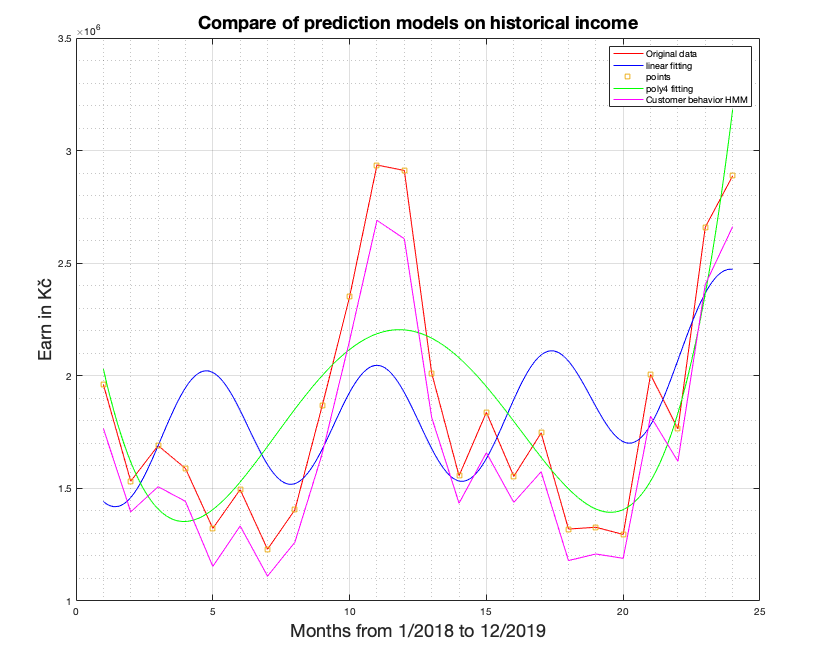
\includegraphics[width=140mm]{plot.png}
    \end{center}
    \caption{Fitting the model on real income from 2018 and 2019}
    \label{plot}
\end{figure}\\
With Megaplay s.r.o employees and heureka e-comerce tool the probability weights were set in form of vector for
Customer behavior HMM which tells about probabilities for each hidden states described in section~\ref{sec:submodels}
Vector have to be updated to square matrix which is used in Customer behavior HMM.
Other industry dependent weights and coefficients were set with Megaplay s.r.o employees, based on their data and experiences as in table~\ref{megaplay_data}.\\
Linear and polynomial models were identified with matlab Curve Fitting toolbox, see parameters in the table~\ref{parameters}.
\newpage
\begin{table}[h!]
    \begin{center}
        \begin{tabular}{ | l | c |}
            \hline
            {\textbf{Variable name}} & \textbf{Result}\\
            \hline
            average day visitors for a predicted month $U_a$& 2357 \\
            perceived value for psychology model & 0.87 \\
            number of orders 2018 - 2019 $O_c$ & 26 530 \\
            Unique products sell $U_p$ & 11048\\
            Customer satisfaction & 90\%\\
            Margin & 0.27\\
            $Q_i$ & 4.12\\
            $Q_1$ & 0.94\\
            Vendor coefficients: & \\
            $\beta$ & 0.7\\
            $\gamma$ & 0.7\\
            $\delta$ & 0.85\\
            \hline
            number of visitors 1/2020 & $31 * U_a$\\
            average earn per order & $\sum Income / O_c$\\
            \overline{Q} & $1/U_p * (U_p/ O_c)$\\
            \overline{P} & $1/U_p * margin$\\
            trust & $1/O_c * O_c/U_a$\\
            \hline
        \end{tabular}
    \end{center}
    \caption{Coefficient and calculated values data from Megaplay s.r.o for Customer behavior HMM}
    \label{megaplay_data}
\end{table}\\
\\
\begin{table}[h!]
    \begin{center}
        \begin{tabular}{ | l | l | l |}
            \hline
            \textbf{linear model} & \textbf{polynomial model} & \textbf{Customer behavior HMM}\\
            \hline
            \makecell{$a =2.978.10^5$\\$b = 1687$\\$c = 1.753.10^6$} & \makecell{$p_1 = 225.1$\\$p_2 = -1.059.10^4$\\$p_3 =1.596.10^5$\\$p_4 = -8.205.10^5$\\$p_5 = 2.702.10^6$} & \makecell{$l = 1/2$\\$m = 1/3$\\$k = 1/9$}\\
            \hline
        \end{tabular}
    \end{center}
    \caption{Identified parameters for models}
    \label{parameters}
\end{table}\\
On the figure~\ref{results} prediction results are shown.
For the year 2021 the models are compared with the real income and we can see that the polynomial and Customer behavior HMM model
get good results, in the opposite of results of linear model prediction.

\begin{figure}[h!]
    \begin{center}
        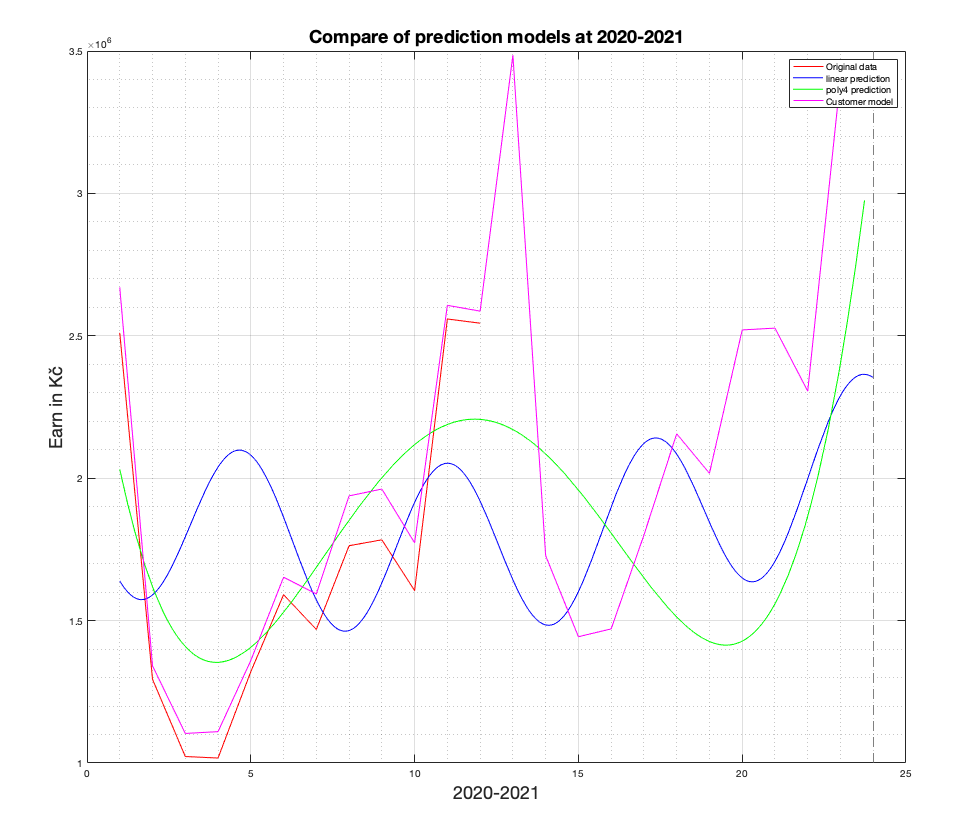
\includegraphics[width=140mm]{results.png}
    \end{center}
    \caption{Prediction from models for years 2020-2021, with real income for 2020.}
    \label{results}
\end{figure}\\
In the graphical view we saw that all our models copy the income, but some of them are easier to calculate, this differences you can see described in Summary (see section~\ref{summary}).
Lets use our defined methodology (see section~\ref{subsec:result_metodology}) to compare our models.
As it given in the table~\ref{compare} our Customer behavior HMM return best results from all tested models.
\begin{table}[h!]
    \begin{center}
        \begin{tabular}{ | l | c | c | c |}
            \hline
            & \textbf{linear model} & \textbf{polynomial model} & \textbf{Customer behavior HMM}\\
            \hline
            \textbf{SSE} & 5,165.10^{12} & 2,534.10^{12} & 1,583.10^{11} \\
            \textbf{R-square} & 0,2162 & 0,6154 & 0,95 \\
            \textbf{RMSE} & 4,959.10^5 & 3,652.10^5 & 1,149.10^5\\
            \hline
        \end{tabular}
    \end{center}
    \caption{Compare goodness-of-fit for models.}
    \label{compare}
\end{table}\\
In the table~\ref{Compare results} calculated percentage aberration from real income in the year 2021 are given.
We saw that there is no model which returned best results in every month, but in most months the best results are offered by Customer behavior HMM.
\begin{table}[h!]
    \begin{center}
        \begin{tabular}{ | l | c | c | c |}
            \hline
            {\textbf{Month}} & \textbf{Linear model} & \textbf{Polynomial model} & \textbf{Customer behavior HMM}\\
            \hline
            1/2021 & 53 & 24 &  7\\
            2/2021 & 23 & 31 & 6\\
            3/2021 & 71 & 38 & 7\\
            4/2021 & 101 & 38 & 13\\
            5/2021 & 57 & 6 & 4\\
            6/2021 & 17 & 5 & 3\\
            7/2021 & 5 & 13 & 7\\
            8/2021 & 20 & 5 & 11\\
            9/2021 & 11 & 11 & 9\\
            10/2021 & 20 & 31 & 10\\
            11/2021 & 25 & 17 & 2\\
            12/2021 & 32 & 16 & 3\\
            \hline
        \end{tabular}
    \end{center}
    \caption{Compare aberration (\%) from real income 2020}
    \label{Compare results}
\end{table}\\
Calculated result per each quarter in 2020 can bee seen in the table~\ref{qResults} showing to us the oscillation of prediction.
\begin{table}[h!]
    \begin{center}
        \begin{tabular}{ | l | c | c | c |}
            \hline
            & \textbf{Linear model} & \textbf{Polynomial model} & \textbf{Customer behavior HMM}\\
            \hline
            1Q (\%) & 49,24 & 30,81 & 6,42\\
            2Q (\%) & 58,24 & 15,00 & 6,50\\
            3Q (\%) & 12,15 & 9,64 & 9,25\\
            4Q (\%) & 25,59 & 21,21 & 4,89\\
            \hline
        \end{tabular}
    \end{center}
    \caption{Quarterly results}
    \label{qResults}
\end{table}\\
\section{Matlab Live script application} \label{livescript}
Implementation of our experiment created in Matlab with results explanations enriched with Live script application with dynamic weights setting is described in this section.
\subsection{Used software, libraries and predefined functions} \label{subsec:libraries}
\textbf{Matlab 2020a}\\
MATLAB (matrix laboratory) is a fourth-generation high-level programming language and interactive environment for numerical
computation, visualization and programming developed by MathWorks.\\
\\
\textbf{Matlab LiveScript}~\cite{livescript}\\
MATLAB live scripts and live functions are interactive documents that combine MATLAB code with formatted text, equations,
and images in a single environment called the Live Editor.
In addition, live scripts store and display output alongside the code that creates it.\\
Use live scripts and functions to:\\
\begin{itemize}
    \item Visually explore and analyze problems.
    \item Share richly formatted, executable narratives.
    \item Create interactive lectures for teaching.
\end{itemize}\\
\\
\textbf{Matlab Curve Fitting Tool}\\
The Curve Fitting Toolbox provides a collection of GUIs and M-files.
With the toolbox we are able to data preprocessing such as sectioning and smoothing, parametric and nonparametric data fitting,
and also fit statistics which assist us in determining the goodness of fit,analysis capabilities such as extrapolation, differentiation, and integration.
A graphical environment allows you to explore and analyze data sets and fits visually and numerically.\\
\textbf{hhmgenerate~\cite{hhmgenerate}}\\
The function $hmmgenerate$ begins with the model in state 1 at step 0, prior to the first emission.
The model then makes a transition to state $i_1$, with probability $T_{1i_1}$, and generates an emission $a_k_1$ with probability $E_{i_1k_11}$.
$hmmgenerate$ returns $i_1$ as the first entry of states, and $a_k_1$ as the first entry of seq.
$[seq,states] = hmmgenerate(len,TRANS,EMIS)$ takes a known Markov model, specified by transition probability matrix $TRANS$ and emission probability matrix $EMIS$,
and uses it to generate:\\
\begin{itemize}
    \item A random sequence seq of emission symbols.
    \item A random sequence states of states.
\end{itemize}
The length of both $seq$ and $states$ is $len$.
$TRANS(i,j)$ is the probability of transition from state $i$ to state $j$.
$EMIS(k,l)$ is the probability that symbol $l$ is emitted from state $k$.\\
\\
\textbf{hhmviterbi}~\cite{hhmviterbi}\\
The function $hmmviterbi$ begins with the model in state 1 at step 0, prior to the first emission.
hmmviterbi computes the most likely path based on the fact that the model begins in state 1.
$STATES = hmmviterbi(seq,TRANS,EMIS)$ given a $sequence, seq$, calculates the most likely path through the hidden Markov model
specified by transition probability matrix, $TRANS$, and emission probability matrix $EMIS$. $TRANS(i,j)$ is the probability of transition from state $i$ to state $j$.
$EMIS(i,k)$ is the probability that symbol $k$ is emitted from state $i$.\\
\\
\textbf{shopycrm.com}\\
Online CRM application focused on e-commerce stores which provides all store workflows and get precalculated data which
we will use for our models to simplify the prediction calculation.
\subsection{Fitting models and prediction} \label{fitting}
Let us use Matlab Curve fitting tool to solve our linear and polynomial models as you can see on figure~\ref{cftool},
this predefined tool calculates coefficients and then the prediction in Matlab Live script was done as we see on figure~\ref{predict}.
These two models were fitted on income data from years 2018 and 2019 as is described in our Experiment (see section~\ref{experiment}).
\begin{figure}[h!]
    \begin{center}
        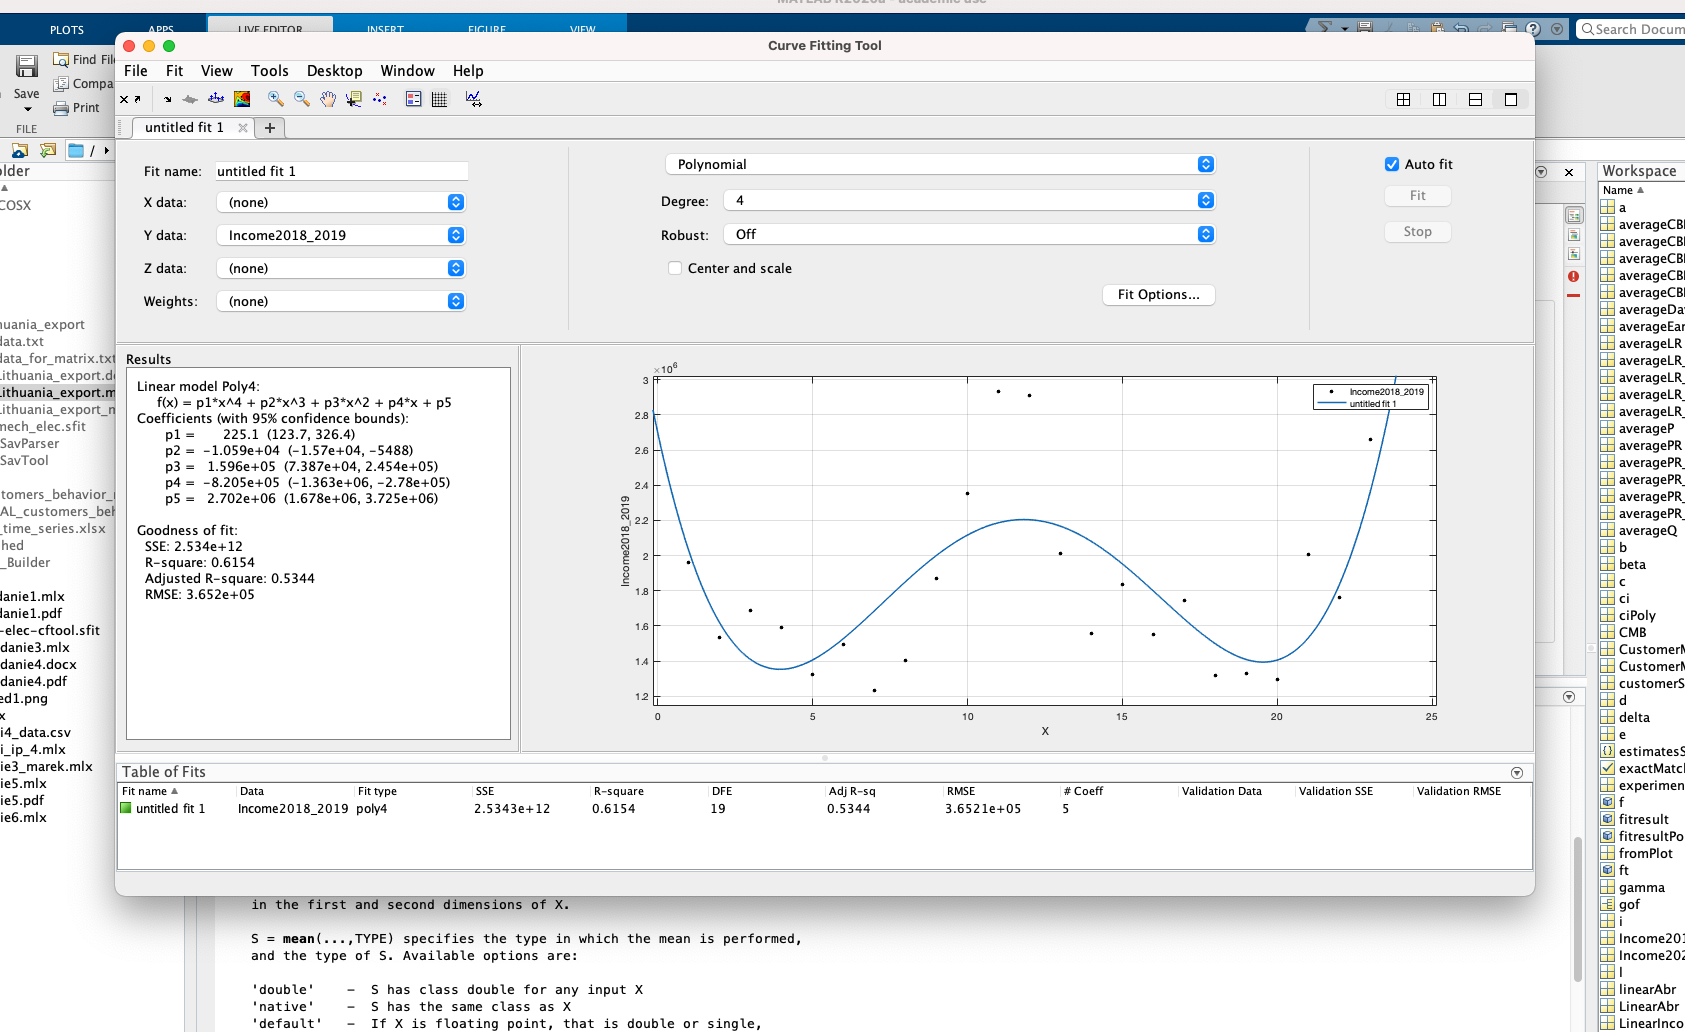
\includegraphics[width=100mm]{cftool.png}
    \end{center}
    \caption{Fitting the data with cftool~\cite{luarn}}
    \label{cftool}
\end{figure}\\
Then to calculate aberration we read the predicted results from the plotted models results as shown on figure~\ref{predict}.
\begin{figure}[h!]
    \begin{center}
        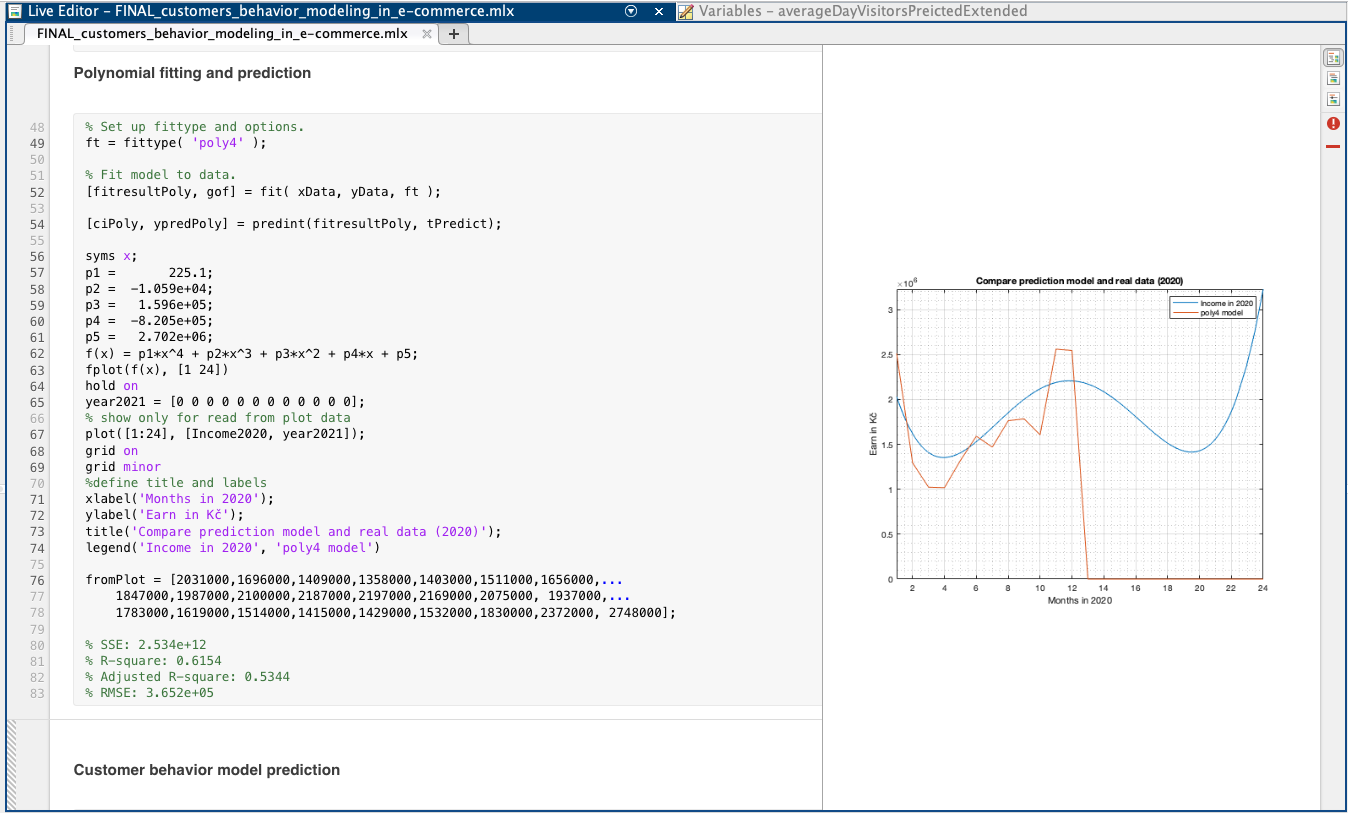
\includegraphics[width=100mm]{predict.png}
    \end{center}
    \caption{Predict income data in live script~\cite{luarn}}
    \label{predict}
\end{figure}\\
\\
Prediction from Customer behavior HMM was made 10 times by default, but this number of cycle run can be easy set in the script.
The final result is arithmetic mean from this prediction which is ten times run to minimize random deviation.
For modeling and dynamic prediction Live scripts Controls are used so in the script we are able to easily set all
constants to model to simulate different situations.
See the dynamic function of our prepared model on figure~\ref{app}.
\begin{figure}[h!]
    \begin{center}
        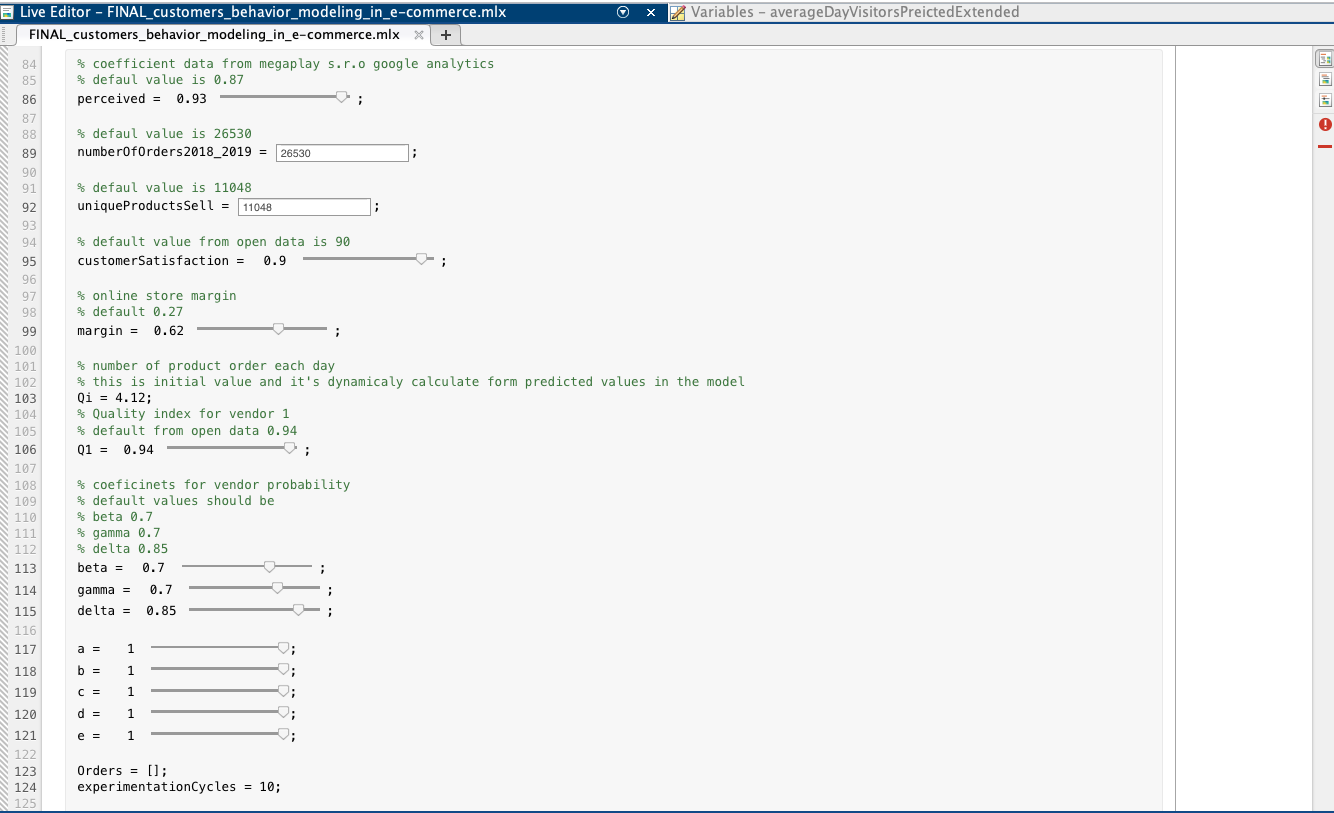
\includegraphics[width=100mm]{app.png}
    \end{center}
    \caption{Live Script application to dynamically set weights and constants for model}
    \label{app}
\end{figure}\\
This precalculated data entered calculation loop.
Next loop reads the value of predefined number of customers in each period and simulates the virtual customer behavior in order process.
This feature gives us ability to easily simulate our model in a different situation.
Lets see some modeled situation in appendix section~\ref{apendixc}.
That results are described in the final summary~\ref{summary} same as results from previous regression models.

% !TEX root = ../thesis.tex

\chapter{Summary} \label{summary}
In our work we focused on creating mathematical models to predict customer behavior based on previous store data and open data available in online tools.
As a baseline we used linear and polynomial regression which is generally used to predict this kind of data.
At the first sight it looks like that the better reference is polynomial model prediction as you can see in the table with results~\ref{results},
but the trend prediction from the simpliest linear regression is useful for some approaches.
Because of simplicity to solve the model.
In case that we have only this two models as a primary goal, it will be good idea to test their cooperation and use one to correct another.
It should generate a very interesting results with trends prediction and income with small aberration too.
Polynomial prediction has in some months worse results than we expected, this was caused by pandemic situation in the predicted year 2020.
This situation was absolutely unpredictable.
However our set goal was to create a better mechanism to predict this important data for each business based on e-commerce solutions.
To pass our goal we used mechanisms for behavior prediction and mathematical approaches which are usually used in other industries like an autonomous driving,
telecommunications or idea which is looking for a correlation between introduce a new products on market with global consumer behavior.
Mechanisms and approaches that we have learned during the work on this thesis give us the ability to create our own vendor,
psychology and loyalty models which are the base for the final prediction model and help us to finish the goal which we have sat at the beginning of the work.
Our main goal was successful prediction with aberration from real income about 6,6\% for the year 2020 and R-square 0,95.
In order to have best results from our model against the other models we would need more time for preparing data to prediction model.
If the polynomial model could use more data for training, it would return better results, but it was not the goal of our work.
Our goal was fulfilled in cooperation with the Megaplay s.r.o which showed us its business and industry and helped set constants for the prediction model with a minimal deflection.
Therefore the next steps should be clearly define mechanisms to set independent industry constants only on ordinary accessible data without consultation with business owners.
Then it will be good to minimize random generated number with a matrix created with real data of store.
We estabilished competitors matrix with real data to compare real store and vendor power and customer satisfaction.
Unfortunately it opens lot of new problems which have to be solved like a vendor strength comparation across industries.
The situation in the industry was change in an unexpected way and modeling such a situation was beyond this thesis.
The results of the thesis are good enough to show that standard simple statistics approaches are not enough for prediction
customer behavior in a 21st century, so we have to look at the sophisticated approaches.
The evolution of computer technology gives the power to get more complicated calculation to more users and it should be used
to get the more relevant data for entrepreneurs to improve their businesses.
Our prediction is actually combination of our models inside statistical solution like Hidden Markov model.
In the future it will be the right way to leave all statics mechanism and as a combination approach use differential equation
which should be able to serve prediction vector to get results lilke a HMM.
However, when this equation will be found, it opens up a new way of predicting store data from predefined states to dynamically
updated states, and displays real-time results to reflect real visitors and revenue in each store.
From different simulation using our script and update constants we get presumed results but not surprising results for us
The number of predicted orders is dependent on numbers of store visitors.
Customer satisfaction with the combination with price index is the most important value for the prediction and it is corespondent
with real behavior, but this is not generally truth.
It can be aplied to our Central Europe region.
However in the future will be better to have data from different countries or continents to check our model in more global way.
We should expect that the weights ratio will be different in other markets, it will depend on psychology of specific customer and behavior in different countries


% good linebraking of bibtex url
\setcounter{biburllcpenalty}{7000}
\setcounter{biburlucpenalty}{8000}

%% The bibliography
\printbibliography[heading=bibintoc]

\label{theend} % the last page of the thesis

% List of acronyms
\printglossary[type=\acronymtype,title={\acrlistname}]

% Glossaries
%\printglossary

%% Appendix
% !TEX root = ../thesis.tex

\chapter*{List of appendix}
\addcontentsline{toc}{chapter}{List of appendix}

\begin{description}
	\item[Appendix A] Reference earn data from Megaplay s.r.o
	\item[Appendix B] Flowcharts
\end{description}

\appendix
\renewcommand\chaptername{Appendix}
% !TEX root = ../thesis.tex

\chapter{Reference data}

As reference will be used Time series analysis and polynomial prediction from Megaplay s.r.o earn data. Data will by exported from their online stores in 2018 and 2019.
Against that results we will be testing our prediction models to have better result and comparing with time series and polynomial prediction.
\subsection{Megaplay s.r.o online stores earn from 2018 and 2019 per months}
\begin{table}[h!]
    \begin{center}
        \begin{tabular}{ | l | c | }
            \hline
            {\textbf{Months}} & \textbf{Earn} \\
            \hline
            1/2018 & 1 961 088 Kč \\
            \hline
            2/2018 & 1 531 995 Kč \\
            \hline
            3/2018 & 1 689 860 Kč \\
            \hline
            4/2018 & 1 588 628 Kč \\
            \hline
            5/2018 & 1 322 548 Kč \\
            \hline
            6/2018 & 1 494 798 Kč \\
            \hline
            7/2018 & 1 229 718 Kč \\
            \hline
            8/2018 & 1 404 787 Kč \\
            \hline
            9/2018 & 1 867 475 Kč \\
            \hline
            10/2018 & 2 350 839 Kč \\
            \hline
            11/2018 & 2 935 847 Kč \\
            \hline
            12/2018 & 2 911 601 Kč \\
            \hline
        \end{tabular}
    \end{center}
    \caption{Megaplay s.r.o earns from 2018}
    \label{Megaplay s.r.o earns from 2018}
\end{table}
\newpage
\begin{table}[h!]
    \begin{center}
        \begin{tabular}{ | l | c | }
            \hline
            1/2019 & 2 012 000 Kč \\
            \hline
            2/2019 & 1 555 929 Kč \\
            \hline
            3/2019 & 1 837 794 Kč \\
            \hline
            4/2019 & 1 553 459 Kč \\
            \hline
            5/2019 & 1 746 159 Kč \\
            \hline
            6/2019 & 1 319 472 Kč \\
            \hline
            7/2019 & 1 327 479 Kč \\
            \hline
            8/2019 & 1 295 468 Kč \\
            \hline
            9/2019 & 2 005 098 Kč \\
            \hline
            10/2019 & 1 763 850 Kč \\
            \hline
            11/2019 & 2 660 196 Kč \\
            \hline
            12/2019 & 2 887 786 Kč \\
            \hline
        \end{tabular}
    \end{center}
    \caption{Megaplay s.r.o earns from 2019}
    \label{Megaplay s.r.o earns from 2019}
\end{table}

% !TEX root = ../thesis.tex

\chapter{Flowcharts}

\section{Overview}
\begin{figure}[h!]
    \begin{center}
        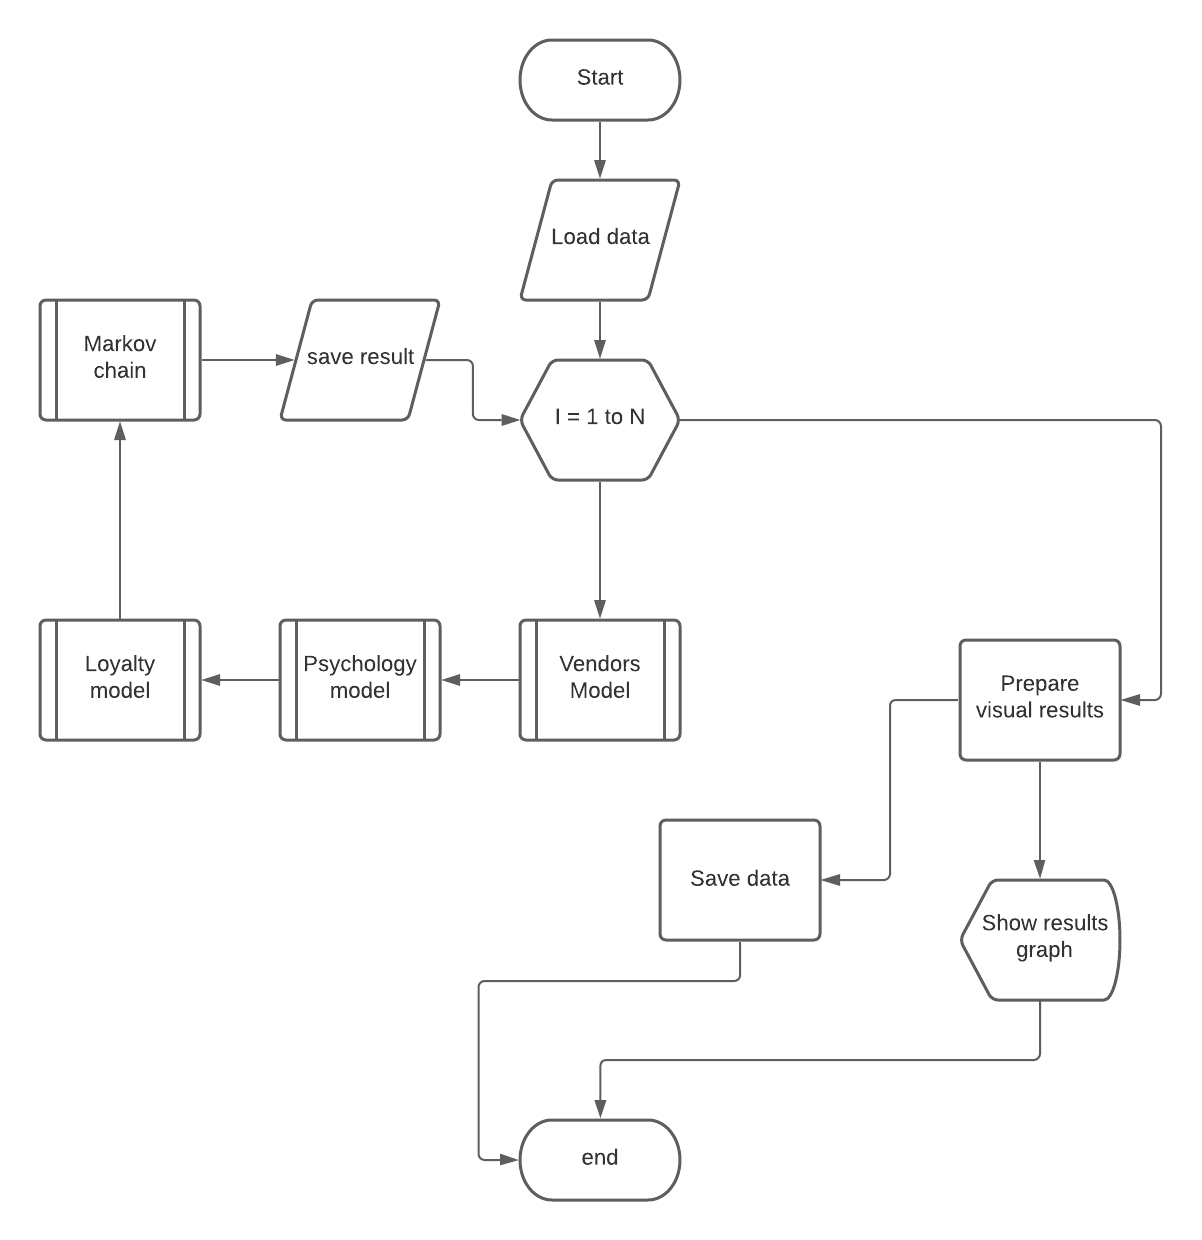
\includegraphics[width=350]{flowchart_overview}
    \end{center}
    \caption{Flowchart overview}
    \label{flowchart_overview}
\end{figure}
\newpage
\section{Vendor model}
\begin{figure}[h!]
    \begin{center}
        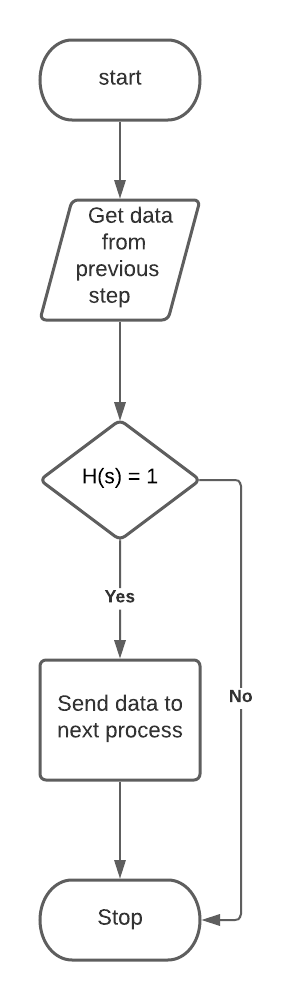
\includegraphics[width=180]{flowchart_vendor}
    \end{center}
    \caption{Flowchart vendor model}
    \label{flowchart_vendor}
\end{figure}
\section{Psychology model}
\begin{figure}[h!]
    \begin{center}
        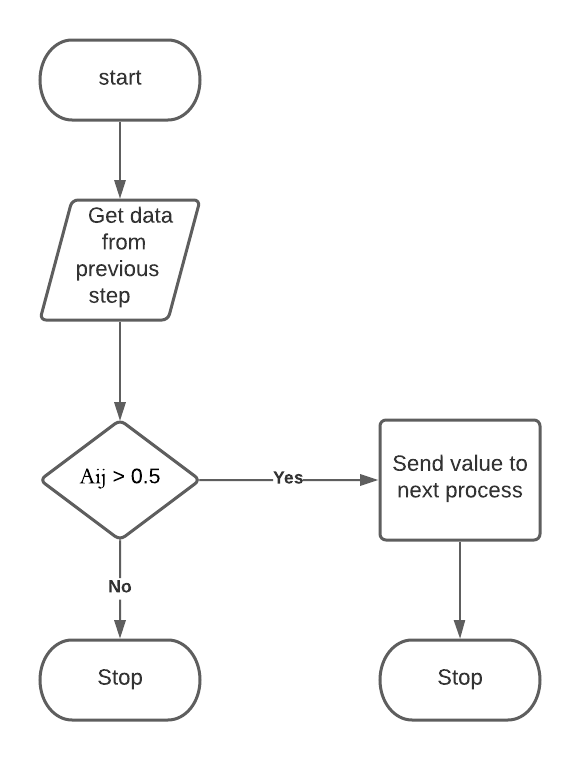
\includegraphics[width=180]{flowchart_psychology}
    \end{center}
    \caption{Flowchart psychology model}
    \label{flowchart_psychology}
\end{figure}
\newpage
\section{Loyalty model}
\begin{figure}[h!]
    \begin{center}
        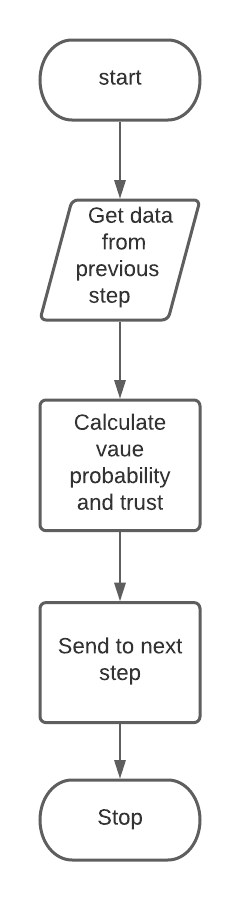
\includegraphics[width=60]{flowchart_loyalty}
    \end{center}
    \caption{Flowchart loyalty model}
    \label{flowchart_loyalty}
\end{figure}
\section{Markov hidden model}
\begin{figure}[h!]
    \begin{center}
        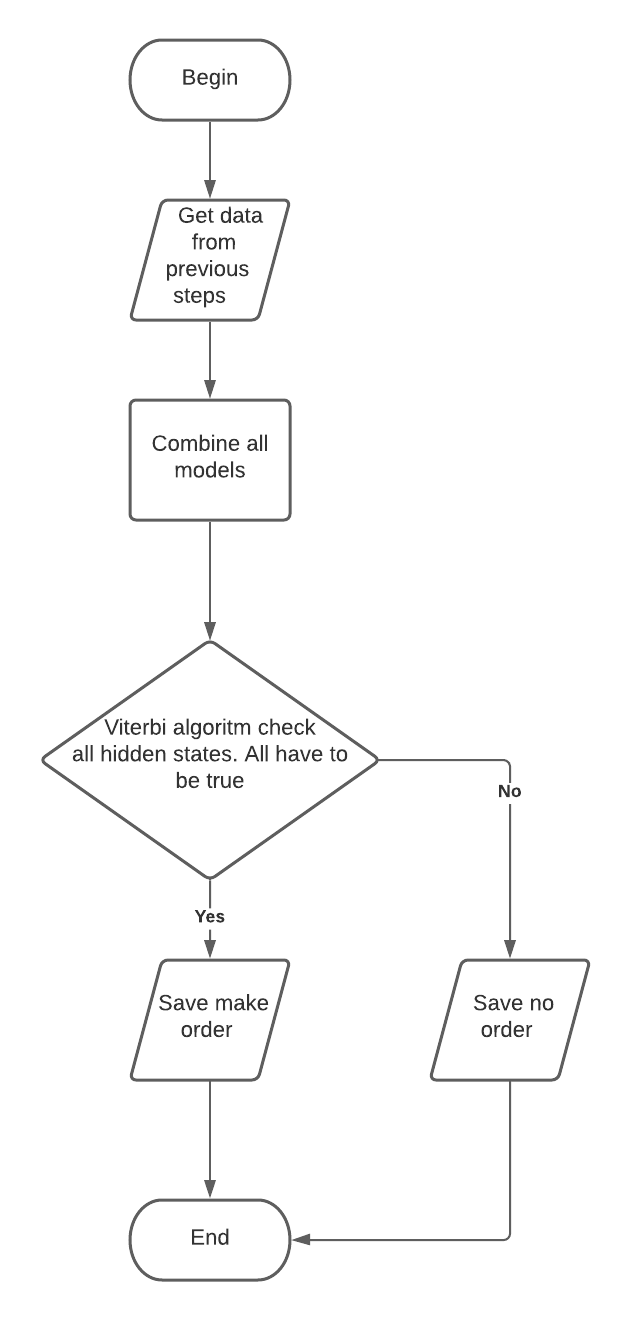
\includegraphics[width=230]{flowchart_markovpng}
    \end{center}
    \caption{Flowchart markov chain}
    \label{flowchart_markov}
\end{figure}
\newpage


% zivotopis autora
%\curriculumvitae\protect
%Táto časť\/ je nepovinná. Autor tu môže uviesť\/ svoje biografické
%údaje, údaje o~záujmoch, účasti na~projektoch, účasti na~súťažiach,
%získané ocenenia, zahraničné pobyty na~praxi, domácu prax, publikácie
%a~pod.

\end{document}
